
% Default to the notebook output style

    


% Inherit from the specified cell style.




    
\documentclass[11pt]{article}

    
    
    \usepackage[T1]{fontenc}
    % Nicer default font (+ math font) than Computer Modern for most use cases
    \usepackage{mathpazo}

    % Basic figure setup, for now with no caption control since it's done
    % automatically by Pandoc (which extracts ![](path) syntax from Markdown).
    \usepackage{graphicx}
    % We will generate all images so they have a width \maxwidth. This means
    % that they will get their normal width if they fit onto the page, but
    % are scaled down if they would overflow the margins.
    \makeatletter
    \def\maxwidth{\ifdim\Gin@nat@width>\linewidth\linewidth
    \else\Gin@nat@width\fi}
    \makeatother
    \let\Oldincludegraphics\includegraphics
    % Set max figure width to be 80% of text width, for now hardcoded.
    \renewcommand{\includegraphics}[1]{\Oldincludegraphics[width=.8\maxwidth]{#1}}
    % Ensure that by default, figures have no caption (until we provide a
    % proper Figure object with a Caption API and a way to capture that
    % in the conversion process - todo).
    \usepackage{caption}
    \DeclareCaptionLabelFormat{nolabel}{}
    \captionsetup{labelformat=nolabel}

    \usepackage{adjustbox} % Used to constrain images to a maximum size 
    \usepackage{xcolor} % Allow colors to be defined
    \usepackage{enumerate} % Needed for markdown enumerations to work
    \usepackage{geometry} % Used to adjust the document margins
    \usepackage{amsmath} % Equations
    \usepackage{amssymb} % Equations
    \usepackage{textcomp} % defines textquotesingle
    % Hack from http://tex.stackexchange.com/a/47451/13684:
    \AtBeginDocument{%
        \def\PYZsq{\textquotesingle}% Upright quotes in Pygmentized code
    }
    \usepackage{upquote} % Upright quotes for verbatim code
    \usepackage{eurosym} % defines \euro
    \usepackage[mathletters]{ucs} % Extended unicode (utf-8) support
    \usepackage[utf8x]{inputenc} % Allow utf-8 characters in the tex document
    \usepackage{fancyvrb} % verbatim replacement that allows latex
    \usepackage{grffile} % extends the file name processing of package graphics 
                         % to support a larger range 
    % The hyperref package gives us a pdf with properly built
    % internal navigation ('pdf bookmarks' for the table of contents,
    % internal cross-reference links, web links for URLs, etc.)
    \usepackage{hyperref}
    \usepackage{longtable} % longtable support required by pandoc >1.10
    \usepackage{booktabs}  % table support for pandoc > 1.12.2
    \usepackage[inline]{enumitem} % IRkernel/repr support (it uses the enumerate* environment)
    \usepackage[normalem]{ulem} % ulem is needed to support strikethroughs (\sout)
                                % normalem makes italics be italics, not underlines
    

    
    
    % Colors for the hyperref package
    \definecolor{urlcolor}{rgb}{0,.145,.698}
    \definecolor{linkcolor}{rgb}{.71,0.21,0.01}
    \definecolor{citecolor}{rgb}{.12,.54,.11}

    % ANSI colors
    \definecolor{ansi-black}{HTML}{3E424D}
    \definecolor{ansi-black-intense}{HTML}{282C36}
    \definecolor{ansi-red}{HTML}{E75C58}
    \definecolor{ansi-red-intense}{HTML}{B22B31}
    \definecolor{ansi-green}{HTML}{00A250}
    \definecolor{ansi-green-intense}{HTML}{007427}
    \definecolor{ansi-yellow}{HTML}{DDB62B}
    \definecolor{ansi-yellow-intense}{HTML}{B27D12}
    \definecolor{ansi-blue}{HTML}{208FFB}
    \definecolor{ansi-blue-intense}{HTML}{0065CA}
    \definecolor{ansi-magenta}{HTML}{D160C4}
    \definecolor{ansi-magenta-intense}{HTML}{A03196}
    \definecolor{ansi-cyan}{HTML}{60C6C8}
    \definecolor{ansi-cyan-intense}{HTML}{258F8F}
    \definecolor{ansi-white}{HTML}{C5C1B4}
    \definecolor{ansi-white-intense}{HTML}{A1A6B2}

    % commands and environments needed by pandoc snippets
    % extracted from the output of `pandoc -s`
    \providecommand{\tightlist}{%
      \setlength{\itemsep}{0pt}\setlength{\parskip}{0pt}}
    \DefineVerbatimEnvironment{Highlighting}{Verbatim}{commandchars=\\\{\}}
    % Add ',fontsize=\small' for more characters per line
    \newenvironment{Shaded}{}{}
    \newcommand{\KeywordTok}[1]{\textcolor[rgb]{0.00,0.44,0.13}{\textbf{{#1}}}}
    \newcommand{\DataTypeTok}[1]{\textcolor[rgb]{0.56,0.13,0.00}{{#1}}}
    \newcommand{\DecValTok}[1]{\textcolor[rgb]{0.25,0.63,0.44}{{#1}}}
    \newcommand{\BaseNTok}[1]{\textcolor[rgb]{0.25,0.63,0.44}{{#1}}}
    \newcommand{\FloatTok}[1]{\textcolor[rgb]{0.25,0.63,0.44}{{#1}}}
    \newcommand{\CharTok}[1]{\textcolor[rgb]{0.25,0.44,0.63}{{#1}}}
    \newcommand{\StringTok}[1]{\textcolor[rgb]{0.25,0.44,0.63}{{#1}}}
    \newcommand{\CommentTok}[1]{\textcolor[rgb]{0.38,0.63,0.69}{\textit{{#1}}}}
    \newcommand{\OtherTok}[1]{\textcolor[rgb]{0.00,0.44,0.13}{{#1}}}
    \newcommand{\AlertTok}[1]{\textcolor[rgb]{1.00,0.00,0.00}{\textbf{{#1}}}}
    \newcommand{\FunctionTok}[1]{\textcolor[rgb]{0.02,0.16,0.49}{{#1}}}
    \newcommand{\RegionMarkerTok}[1]{{#1}}
    \newcommand{\ErrorTok}[1]{\textcolor[rgb]{1.00,0.00,0.00}{\textbf{{#1}}}}
    \newcommand{\NormalTok}[1]{{#1}}
    
    % Additional commands for more recent versions of Pandoc
    \newcommand{\ConstantTok}[1]{\textcolor[rgb]{0.53,0.00,0.00}{{#1}}}
    \newcommand{\SpecialCharTok}[1]{\textcolor[rgb]{0.25,0.44,0.63}{{#1}}}
    \newcommand{\VerbatimStringTok}[1]{\textcolor[rgb]{0.25,0.44,0.63}{{#1}}}
    \newcommand{\SpecialStringTok}[1]{\textcolor[rgb]{0.73,0.40,0.53}{{#1}}}
    \newcommand{\ImportTok}[1]{{#1}}
    \newcommand{\DocumentationTok}[1]{\textcolor[rgb]{0.73,0.13,0.13}{\textit{{#1}}}}
    \newcommand{\AnnotationTok}[1]{\textcolor[rgb]{0.38,0.63,0.69}{\textbf{\textit{{#1}}}}}
    \newcommand{\CommentVarTok}[1]{\textcolor[rgb]{0.38,0.63,0.69}{\textbf{\textit{{#1}}}}}
    \newcommand{\VariableTok}[1]{\textcolor[rgb]{0.10,0.09,0.49}{{#1}}}
    \newcommand{\ControlFlowTok}[1]{\textcolor[rgb]{0.00,0.44,0.13}{\textbf{{#1}}}}
    \newcommand{\OperatorTok}[1]{\textcolor[rgb]{0.40,0.40,0.40}{{#1}}}
    \newcommand{\BuiltInTok}[1]{{#1}}
    \newcommand{\ExtensionTok}[1]{{#1}}
    \newcommand{\PreprocessorTok}[1]{\textcolor[rgb]{0.74,0.48,0.00}{{#1}}}
    \newcommand{\AttributeTok}[1]{\textcolor[rgb]{0.49,0.56,0.16}{{#1}}}
    \newcommand{\InformationTok}[1]{\textcolor[rgb]{0.38,0.63,0.69}{\textbf{\textit{{#1}}}}}
    \newcommand{\WarningTok}[1]{\textcolor[rgb]{0.38,0.63,0.69}{\textbf{\textit{{#1}}}}}
    
    
    % Define a nice break command that doesn't care if a line doesn't already
    % exist.
    \def\br{\hspace*{\fill} \\* }
    % Math Jax compatability definitions
    \def\gt{>}
    \def\lt{<}
    % Document parameters
    \title{worksheet\_01}
    
    
    

    % Pygments definitions
    
\makeatletter
\def\PY@reset{\let\PY@it=\relax \let\PY@bf=\relax%
    \let\PY@ul=\relax \let\PY@tc=\relax%
    \let\PY@bc=\relax \let\PY@ff=\relax}
\def\PY@tok#1{\csname PY@tok@#1\endcsname}
\def\PY@toks#1+{\ifx\relax#1\empty\else%
    \PY@tok{#1}\expandafter\PY@toks\fi}
\def\PY@do#1{\PY@bc{\PY@tc{\PY@ul{%
    \PY@it{\PY@bf{\PY@ff{#1}}}}}}}
\def\PY#1#2{\PY@reset\PY@toks#1+\relax+\PY@do{#2}}

\expandafter\def\csname PY@tok@w\endcsname{\def\PY@tc##1{\textcolor[rgb]{0.73,0.73,0.73}{##1}}}
\expandafter\def\csname PY@tok@c\endcsname{\let\PY@it=\textit\def\PY@tc##1{\textcolor[rgb]{0.25,0.50,0.50}{##1}}}
\expandafter\def\csname PY@tok@cp\endcsname{\def\PY@tc##1{\textcolor[rgb]{0.74,0.48,0.00}{##1}}}
\expandafter\def\csname PY@tok@k\endcsname{\let\PY@bf=\textbf\def\PY@tc##1{\textcolor[rgb]{0.00,0.50,0.00}{##1}}}
\expandafter\def\csname PY@tok@kp\endcsname{\def\PY@tc##1{\textcolor[rgb]{0.00,0.50,0.00}{##1}}}
\expandafter\def\csname PY@tok@kt\endcsname{\def\PY@tc##1{\textcolor[rgb]{0.69,0.00,0.25}{##1}}}
\expandafter\def\csname PY@tok@o\endcsname{\def\PY@tc##1{\textcolor[rgb]{0.40,0.40,0.40}{##1}}}
\expandafter\def\csname PY@tok@ow\endcsname{\let\PY@bf=\textbf\def\PY@tc##1{\textcolor[rgb]{0.67,0.13,1.00}{##1}}}
\expandafter\def\csname PY@tok@nb\endcsname{\def\PY@tc##1{\textcolor[rgb]{0.00,0.50,0.00}{##1}}}
\expandafter\def\csname PY@tok@nf\endcsname{\def\PY@tc##1{\textcolor[rgb]{0.00,0.00,1.00}{##1}}}
\expandafter\def\csname PY@tok@nc\endcsname{\let\PY@bf=\textbf\def\PY@tc##1{\textcolor[rgb]{0.00,0.00,1.00}{##1}}}
\expandafter\def\csname PY@tok@nn\endcsname{\let\PY@bf=\textbf\def\PY@tc##1{\textcolor[rgb]{0.00,0.00,1.00}{##1}}}
\expandafter\def\csname PY@tok@ne\endcsname{\let\PY@bf=\textbf\def\PY@tc##1{\textcolor[rgb]{0.82,0.25,0.23}{##1}}}
\expandafter\def\csname PY@tok@nv\endcsname{\def\PY@tc##1{\textcolor[rgb]{0.10,0.09,0.49}{##1}}}
\expandafter\def\csname PY@tok@no\endcsname{\def\PY@tc##1{\textcolor[rgb]{0.53,0.00,0.00}{##1}}}
\expandafter\def\csname PY@tok@nl\endcsname{\def\PY@tc##1{\textcolor[rgb]{0.63,0.63,0.00}{##1}}}
\expandafter\def\csname PY@tok@ni\endcsname{\let\PY@bf=\textbf\def\PY@tc##1{\textcolor[rgb]{0.60,0.60,0.60}{##1}}}
\expandafter\def\csname PY@tok@na\endcsname{\def\PY@tc##1{\textcolor[rgb]{0.49,0.56,0.16}{##1}}}
\expandafter\def\csname PY@tok@nt\endcsname{\let\PY@bf=\textbf\def\PY@tc##1{\textcolor[rgb]{0.00,0.50,0.00}{##1}}}
\expandafter\def\csname PY@tok@nd\endcsname{\def\PY@tc##1{\textcolor[rgb]{0.67,0.13,1.00}{##1}}}
\expandafter\def\csname PY@tok@s\endcsname{\def\PY@tc##1{\textcolor[rgb]{0.73,0.13,0.13}{##1}}}
\expandafter\def\csname PY@tok@sd\endcsname{\let\PY@it=\textit\def\PY@tc##1{\textcolor[rgb]{0.73,0.13,0.13}{##1}}}
\expandafter\def\csname PY@tok@si\endcsname{\let\PY@bf=\textbf\def\PY@tc##1{\textcolor[rgb]{0.73,0.40,0.53}{##1}}}
\expandafter\def\csname PY@tok@se\endcsname{\let\PY@bf=\textbf\def\PY@tc##1{\textcolor[rgb]{0.73,0.40,0.13}{##1}}}
\expandafter\def\csname PY@tok@sr\endcsname{\def\PY@tc##1{\textcolor[rgb]{0.73,0.40,0.53}{##1}}}
\expandafter\def\csname PY@tok@ss\endcsname{\def\PY@tc##1{\textcolor[rgb]{0.10,0.09,0.49}{##1}}}
\expandafter\def\csname PY@tok@sx\endcsname{\def\PY@tc##1{\textcolor[rgb]{0.00,0.50,0.00}{##1}}}
\expandafter\def\csname PY@tok@m\endcsname{\def\PY@tc##1{\textcolor[rgb]{0.40,0.40,0.40}{##1}}}
\expandafter\def\csname PY@tok@gh\endcsname{\let\PY@bf=\textbf\def\PY@tc##1{\textcolor[rgb]{0.00,0.00,0.50}{##1}}}
\expandafter\def\csname PY@tok@gu\endcsname{\let\PY@bf=\textbf\def\PY@tc##1{\textcolor[rgb]{0.50,0.00,0.50}{##1}}}
\expandafter\def\csname PY@tok@gd\endcsname{\def\PY@tc##1{\textcolor[rgb]{0.63,0.00,0.00}{##1}}}
\expandafter\def\csname PY@tok@gi\endcsname{\def\PY@tc##1{\textcolor[rgb]{0.00,0.63,0.00}{##1}}}
\expandafter\def\csname PY@tok@gr\endcsname{\def\PY@tc##1{\textcolor[rgb]{1.00,0.00,0.00}{##1}}}
\expandafter\def\csname PY@tok@ge\endcsname{\let\PY@it=\textit}
\expandafter\def\csname PY@tok@gs\endcsname{\let\PY@bf=\textbf}
\expandafter\def\csname PY@tok@gp\endcsname{\let\PY@bf=\textbf\def\PY@tc##1{\textcolor[rgb]{0.00,0.00,0.50}{##1}}}
\expandafter\def\csname PY@tok@go\endcsname{\def\PY@tc##1{\textcolor[rgb]{0.53,0.53,0.53}{##1}}}
\expandafter\def\csname PY@tok@gt\endcsname{\def\PY@tc##1{\textcolor[rgb]{0.00,0.27,0.87}{##1}}}
\expandafter\def\csname PY@tok@err\endcsname{\def\PY@bc##1{\setlength{\fboxsep}{0pt}\fcolorbox[rgb]{1.00,0.00,0.00}{1,1,1}{\strut ##1}}}
\expandafter\def\csname PY@tok@kc\endcsname{\let\PY@bf=\textbf\def\PY@tc##1{\textcolor[rgb]{0.00,0.50,0.00}{##1}}}
\expandafter\def\csname PY@tok@kd\endcsname{\let\PY@bf=\textbf\def\PY@tc##1{\textcolor[rgb]{0.00,0.50,0.00}{##1}}}
\expandafter\def\csname PY@tok@kn\endcsname{\let\PY@bf=\textbf\def\PY@tc##1{\textcolor[rgb]{0.00,0.50,0.00}{##1}}}
\expandafter\def\csname PY@tok@kr\endcsname{\let\PY@bf=\textbf\def\PY@tc##1{\textcolor[rgb]{0.00,0.50,0.00}{##1}}}
\expandafter\def\csname PY@tok@bp\endcsname{\def\PY@tc##1{\textcolor[rgb]{0.00,0.50,0.00}{##1}}}
\expandafter\def\csname PY@tok@fm\endcsname{\def\PY@tc##1{\textcolor[rgb]{0.00,0.00,1.00}{##1}}}
\expandafter\def\csname PY@tok@vc\endcsname{\def\PY@tc##1{\textcolor[rgb]{0.10,0.09,0.49}{##1}}}
\expandafter\def\csname PY@tok@vg\endcsname{\def\PY@tc##1{\textcolor[rgb]{0.10,0.09,0.49}{##1}}}
\expandafter\def\csname PY@tok@vi\endcsname{\def\PY@tc##1{\textcolor[rgb]{0.10,0.09,0.49}{##1}}}
\expandafter\def\csname PY@tok@vm\endcsname{\def\PY@tc##1{\textcolor[rgb]{0.10,0.09,0.49}{##1}}}
\expandafter\def\csname PY@tok@sa\endcsname{\def\PY@tc##1{\textcolor[rgb]{0.73,0.13,0.13}{##1}}}
\expandafter\def\csname PY@tok@sb\endcsname{\def\PY@tc##1{\textcolor[rgb]{0.73,0.13,0.13}{##1}}}
\expandafter\def\csname PY@tok@sc\endcsname{\def\PY@tc##1{\textcolor[rgb]{0.73,0.13,0.13}{##1}}}
\expandafter\def\csname PY@tok@dl\endcsname{\def\PY@tc##1{\textcolor[rgb]{0.73,0.13,0.13}{##1}}}
\expandafter\def\csname PY@tok@s2\endcsname{\def\PY@tc##1{\textcolor[rgb]{0.73,0.13,0.13}{##1}}}
\expandafter\def\csname PY@tok@sh\endcsname{\def\PY@tc##1{\textcolor[rgb]{0.73,0.13,0.13}{##1}}}
\expandafter\def\csname PY@tok@s1\endcsname{\def\PY@tc##1{\textcolor[rgb]{0.73,0.13,0.13}{##1}}}
\expandafter\def\csname PY@tok@mb\endcsname{\def\PY@tc##1{\textcolor[rgb]{0.40,0.40,0.40}{##1}}}
\expandafter\def\csname PY@tok@mf\endcsname{\def\PY@tc##1{\textcolor[rgb]{0.40,0.40,0.40}{##1}}}
\expandafter\def\csname PY@tok@mh\endcsname{\def\PY@tc##1{\textcolor[rgb]{0.40,0.40,0.40}{##1}}}
\expandafter\def\csname PY@tok@mi\endcsname{\def\PY@tc##1{\textcolor[rgb]{0.40,0.40,0.40}{##1}}}
\expandafter\def\csname PY@tok@il\endcsname{\def\PY@tc##1{\textcolor[rgb]{0.40,0.40,0.40}{##1}}}
\expandafter\def\csname PY@tok@mo\endcsname{\def\PY@tc##1{\textcolor[rgb]{0.40,0.40,0.40}{##1}}}
\expandafter\def\csname PY@tok@ch\endcsname{\let\PY@it=\textit\def\PY@tc##1{\textcolor[rgb]{0.25,0.50,0.50}{##1}}}
\expandafter\def\csname PY@tok@cm\endcsname{\let\PY@it=\textit\def\PY@tc##1{\textcolor[rgb]{0.25,0.50,0.50}{##1}}}
\expandafter\def\csname PY@tok@cpf\endcsname{\let\PY@it=\textit\def\PY@tc##1{\textcolor[rgb]{0.25,0.50,0.50}{##1}}}
\expandafter\def\csname PY@tok@c1\endcsname{\let\PY@it=\textit\def\PY@tc##1{\textcolor[rgb]{0.25,0.50,0.50}{##1}}}
\expandafter\def\csname PY@tok@cs\endcsname{\let\PY@it=\textit\def\PY@tc##1{\textcolor[rgb]{0.25,0.50,0.50}{##1}}}

\def\PYZbs{\char`\\}
\def\PYZus{\char`\_}
\def\PYZob{\char`\{}
\def\PYZcb{\char`\}}
\def\PYZca{\char`\^}
\def\PYZam{\char`\&}
\def\PYZlt{\char`\<}
\def\PYZgt{\char`\>}
\def\PYZsh{\char`\#}
\def\PYZpc{\char`\%}
\def\PYZdl{\char`\$}
\def\PYZhy{\char`\-}
\def\PYZsq{\char`\'}
\def\PYZdq{\char`\"}
\def\PYZti{\char`\~}
% for compatibility with earlier versions
\def\PYZat{@}
\def\PYZlb{[}
\def\PYZrb{]}
\makeatother


    % Exact colors from NB
    \definecolor{incolor}{rgb}{0.0, 0.0, 0.5}
    \definecolor{outcolor}{rgb}{0.545, 0.0, 0.0}



    
    % Prevent overflowing lines due to hard-to-break entities
    \sloppy 
    % Setup hyperref package
    \hypersetup{
      breaklinks=true,  % so long urls are correctly broken across lines
      colorlinks=true,
      urlcolor=urlcolor,
      linkcolor=linkcolor,
      citecolor=citecolor,
      }
    % Slightly bigger margins than the latex defaults
    
    \geometry{verbose,tmargin=1in,bmargin=1in,lmargin=1in,rmargin=1in}
    
    

    \begin{document}
    
    
    \maketitle
    
    

    
    \section{Worksheet 1: Introduction to Data
Science}\label{worksheet-1-introduction-to-data-science}

Welcome to DSCI 100: Introduction to Data Science!

Each week you will complete a lecture assignment like this one. Before
we get started, there are some administrative details.

You can't learn technical subjects without hands-on practice. The weekly
lecture worksheets and tutorials are an important part of the course.
The lecture worksheets will automatically be collected at the start of
the weekly tutorial. Conversely, the tutorial assigments will
automatically be collected at the start of the weekly lecture. This is
set up so that you are only working on one thing at a time. Attendance
in lectures and tutorials are required. There will be participatory
activities in both the lecture and tutorial to help support your
learning.

Collaborating on lecture worksheets and tutorial assignments is more
than okay -\/- it's encouraged! You should rarely be stuck for more than
a few minutes on questions in lecture or tutorial, so ask a neighbor, TA
or an instructor for help (explaining things is beneficial, too -\/- the
best way to solidify your knowledge of a subject is to explain it).
Please don't just share answers, though. Everyone must submit a copy of
their own work.

You can read more about
\href{https://github.com/UBC-DSCI/dsci-100/blob/master/policies.md}{course
policies} on the \href{https://github.com/UBC-DSCI/dsci-100}{course
website}.

\subsubsection{Lecture and Tutorial Learning
Goals:}\label{lecture-and-tutorial-learning-goals}

After completing this week's lecture and tutorial work, you will be able
to:

\begin{itemize}
\tightlist
\item
  use a Jupyter notebook to execute provided R code
\item
  edit code and markdown cells in a Jupyter notebook
\item
  create new code and markdown cells in a Jupyter notebook
\item
  load the \texttt{tidyverse} library into R
\item
  create new variables and objects in R using the assignment symbol
\item
  use the help and documentation tools in R
\item
  match the names of the following functions from the \texttt{tidyverse}
  library to their documentation descriptions:

  \begin{itemize}
  \tightlist
  \item
    \texttt{read\_csv}
  \item
    \texttt{select}
  \item
    \texttt{mutate}
  \item
    \texttt{filter}
  \item
    \texttt{ggplot}
  \item
    \texttt{aes}
  \end{itemize}
\item
  chain together two functions using the pipe operator,
  \texttt{\%\textgreater{}\%}
\end{itemize}

In this first worksheet you will also learn how to test the answers you
write in this worksheet to assess if you answered questions correctly
before your assignment is collected.

This worksheet covers parts of
\href{https://ubc-dsci.github.io/introduction-to-data-science/chapter2.html}{Chapter
1} of the online textbook. You should read this chapter before
attempting this worksheet.

    \section{1. Jupyter notebooks}\label{jupyter-notebooks}

This webpage is called a Jupyter notebook. A notebook is a place to
write programs and view their results.

\subsection{1.1. Text cells}\label{text-cells}

In a notebook, each rectangle containing text or code is called a
\emph{cell}.

Text cells (like this one) can be edited by double-clicking on them.
They're written in a simple format called
\href{http://daringfireball.net/projects/markdown/syntax}{Markdown} to
add formatting and section headings. You don't need to learn Markdown,
but you might want to.

After you edit a text cell, click the "run cell" button at the top that
looks like ▶\textbar{} to confirm any changes. (Try not to delete the
instructions of the lab.)

    \textbf{Question 1.1.1.} This paragraph is in its own text cell. Try
editing it so that this sentence is the last sentence in the paragraph,
and then click the "run cell" ▶\textbar{} button . This sentence, for
example, should be deleted. So should this one.

    \subsection{1.2. Code cells}\label{code-cells}

Other cells contain code in the R language. Running a code cell will
execute all of the code it contains.

To run the code in a cell, first click on that cell to activate it.
It'll be highlighted with a little green or blue rectangle. Next, either
press Run ▶\textbar{} or hold down the \texttt{shift} key and press
\texttt{return} or \texttt{enter}.

Try running the next cell:

    \begin{Verbatim}[commandchars=\\\{\}]
{\color{incolor}In [{\color{incolor}1}]:} \PY{k+kp}{print}\PY{p}{(}\PY{l+s}{\PYZdq{}}\PY{l+s}{Hello, World!\PYZdq{}}\PY{p}{)}
\end{Verbatim}


    \begin{Verbatim}[commandchars=\\\{\}]
[1] "Hello, World!"

    \end{Verbatim}

    The above code cell contains a single line of code, but cells can also
contain multiple lines of code. When you run a cell, the lines of code
are executed in the order in which they appear. Every \texttt{print}
expression prints a line. Run the next cell and notice the order of the
output.

    \begin{Verbatim}[commandchars=\\\{\}]
{\color{incolor}In [{\color{incolor}2}]:} \PY{k+kp}{print}\PY{p}{(}\PY{l+s}{\PYZdq{}}\PY{l+s}{First this line is printed,\PYZdq{}}\PY{p}{)}
        \PY{k+kp}{print}\PY{p}{(}\PY{l+s}{\PYZdq{}}\PY{l+s}{and then this one.\PYZdq{}}\PY{p}{)}
\end{Verbatim}


    \begin{Verbatim}[commandchars=\\\{\}]
[1] "First this line is printed,"
[1] "and then this one."

    \end{Verbatim}

    \textbf{Question 1.2.1.} Change the cell above so that it prints out:

\begin{verbatim}
First this line is printed,
and then the next line, 
and then this one.
\end{verbatim}

\emph{Hint:} If you're stuck for more than a few minutes, try talking to
a neighbor or a TA. That's a good idea for any worksheet or tutorial
problem.

    \subsection{1.3. Writing Jupyter
notebooks}\label{writing-jupyter-notebooks}

You can use Jupyter notebooks for your own projects or documents. When
you make your own notebook, you'll need to create your own cells for
text and code.

To add a cell, click the + button in the menu bar. It'll start out as a
code cell. You can change it to a text cell by clicking inside it so
it's highlighted, clicking the drop-down box next to the restart (⟳)
button in the menu bar, and choosing "Markdown".

\textbf{Question 1.3.1.} Add a code cell below this one. Write code in
it that prints out:

\begin{verbatim}
A whole new code cell!
\end{verbatim}

Run your cell to verify that it works.

    \textbf{Question 1.3.2.} Add a text/Markdown cell below this one. Write
the text "A whole new Markdown cell" in it.

    \subsection{1.4. Errors}\label{errors}

R is a language, and like natural human languages, it has rules. It
differs from natural language in two important ways: 1. The rules are
\emph{simple}. You can learn most of them in a few weeks and gain
reasonable proficiency with the language in a semester. 2. The rules are
\emph{rigid}. If you're proficient in a natural language, you can
understand a non-proficient speaker, glossing over small mistakes. A
computer running R code is not smart enough to do that.

Whenever you write code, you'll make mistakes (everyone who writes code
does, even your course instructor!). When you run a code cell that has
errors, R will sometimes produce error messages to tell you what you did
wrong.

Errors are okay; even experienced programmers make many errors. When you
make an error, you just have to find the source of the problem, fix it,
and move on.

We have made an error in the next cell. Run it and see what happens.

    \begin{Verbatim}[commandchars=\\\{\}]
{\color{incolor}In [{\color{incolor}3}]:} \PY{k+kp}{print}\PY{p}{(}\PY{l+s}{\PYZdq{}}\PY{l+s}{This line is missing something.\PYZdq{}}
\end{Verbatim}


    \begin{Verbatim}[commandchars=\\\{\}]

        Error in parse(text = x, srcfile = src): <text>:2:0: unexpected end of input
    1: print("This line is missing something."
       \^{}
    Traceback:


    \end{Verbatim}

    \begin{figure}
\centering
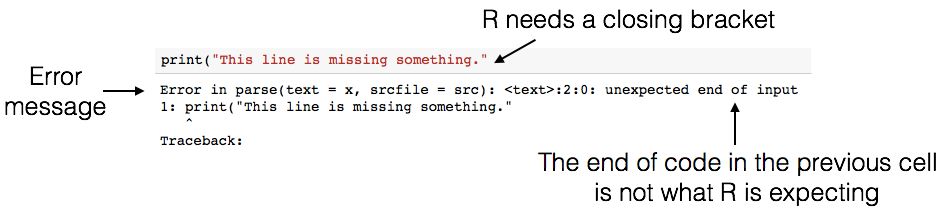
\includegraphics{images/ws1_error_image.png}
\caption{ws1\_error\_image.png}
\end{figure}

    There's a lot of terminology in programming languages, but you don't
need to know it all in order to program effectively. If you see a
cryptic message like this, you can often get by without deciphering it.
(Of course, if you're frustrated, ask a neighbor or a TA for help.)

Try to fix the code above so that you can run the cell and see the
intended message instead of an error.

    \subsection{1.5. The Kernel}\label{the-kernel}

The kernel is a program that executes the code inside your notebook and
outputs the results. In the top right of your window, you can see a
circle that indicates the status of your kernel. If the circle is empty
(⚪), the kernel is idle and ready to execute code. If the circle is
filled in (⚫), the kernel is busy running some code.

You may run into problems where your kernel is stuck for an excessive
amount of time, your notebook is very slow and unresponsive, or your
kernel loses its connection. If this happens, try the following steps:
1. At the top of your screen, click \textbf{Kernel}, then
\textbf{Interrupt}. 2. If that doesn't help, click \textbf{Kernel}, then
\textbf{Restart}. If you do this, you will have to run your code cells
from the start of your notebook up until where you paused your work. 3.
If that doesn't help, restart your server. First, save your work by
clicking \textbf{File} at the top left of your screen, then \textbf{Save
and Checkpoint}. Next, click \textbf{Control Panel} at the top right.
Choose \textbf{Stop My Server} to shut it down, then \textbf{My Server}
to start it back up. Then, navigate back to the notebook you were
working on.

    \subsection{1.6. Submitting your work}\label{submitting-your-work}

All lecture worksheets and tutorials assignments in the course will be
distributed as notebooks like this one. You will complete your work in
this notebook and at the due date we will copy this notebook and grade
that copy. For lecture worksheets we will use a system called nbgrader
that checks your work. For tutorial assignments we will use a
combination of nbgrader and manual grading of your work.

    \section{2. Numbers}\label{numbers}

Quantitative information arises everywhere in data science. In addition
to representing commands to print out lines, our R code can represent
numbers and methods of combining numbers. The expression \texttt{3.2500}
evaluates to the number 3.25. (Run the cell and see.)

    \begin{Verbatim}[commandchars=\\\{\}]
{\color{incolor}In [{\color{incolor}4}]:} \PY{l+m}{3.2500}
\end{Verbatim}


    3.25

    
    Notice that we didn't have to print. When you run a notebook cell,
Jupyter helpfully prints out that value for you.

    \begin{Verbatim}[commandchars=\\\{\}]
{\color{incolor}In [{\color{incolor}5}]:} \PY{l+m}{2}
        \PY{l+m}{3}
        \PY{l+m}{4}
\end{Verbatim}


    2

    
    3

    
    4

    
    Above, you should see that the three numbers (2, 3, and 4) are printed
out. In R, simply inputting numbers and running the cell will generate
all the numbers that you listed. Even though we don't need to use print,
we will continue to do in several places in these worksheets so that we
are very clear with our intentions.

    \subsection{2.1. Arithmetic}\label{arithmetic}

The line in the next cell subtracts. Its value is what you'd expect. Run
it.

    \begin{Verbatim}[commandchars=\\\{\}]
{\color{incolor}In [{\color{incolor}6}]:} \PY{l+m}{2.0} \PY{o}{\PYZhy{}} \PY{l+m}{1.5}
\end{Verbatim}


    0.5

    
    Same with the cell below. Run it.

    \begin{Verbatim}[commandchars=\\\{\}]
{\color{incolor}In [{\color{incolor}7}]:} \PY{l+m}{2} \PY{o}{*} \PY{l+m}{2}
\end{Verbatim}


    4

    
    Many basic arithmetic operations are built in to R.
\href{https://www.statmethods.net/management/operators.html}{This
webpage} describes all the arithmetic operators used in the course. You
can refer back to this webpage as you need throughout the term.

    \section{3. Names}\label{names}

In natural language, we have terminology that lets us quickly reference
very complicated concepts. We don't say, "That's a large mammal with
brown fur and sharp teeth!" Instead, we just say, "Bear!"

Similarly, an effective strategy for writing code is to define names for
data as we compute it, like a lawyer would define terms for complex
ideas at the start of a legal document to simplify the rest of the
writing.

In R, we do this with \emph{objects}. An object has a name on the left
side of an \texttt{\textless{}-} sign and an expression to be evaluated
on the right.

    \begin{Verbatim}[commandchars=\\\{\}]
{\color{incolor}In [{\color{incolor}8}]:} answer \PY{o}{\PYZlt{}\PYZhy{}} \PY{l+m}{3} \PY{o}{*} \PY{l+m}{2} \PY{o}{+} \PY{l+m}{4}
\end{Verbatim}


    When you run that cell, R first evaluates the first line. It computes
the value of the expression \texttt{3\ *\ 2\ +\ 4}, which is the number
10. Then it gives that value the name \texttt{answer}. At that point,
the code in the cell is done running.

After you run that cell, the value 10 is bound to the name
\texttt{answer}:

    \begin{Verbatim}[commandchars=\\\{\}]
{\color{incolor}In [{\color{incolor}9}]:} answer
\end{Verbatim}


    10

    
    We can name our objects anything we'd like. Above we called it
\texttt{answer}, but we could have named it \texttt{value},
\texttt{data} or anything else we desired. A good rule of thumb is to
name it something that has meaning to a human as it relates to what we
are trying to accomplish with our R code.

\textbf{Question 3.1.} Enter a new code cell. Try creating another
object using \texttt{\textless{}-\ 3\ *\ 2\ +\ 4} with a name different
from \texttt{answer}.

    A common pattern in Jupyter notebooks is to assign a value to a name and
then immediately evaluate the name in the last line in the cell so that
the value is displayed as output.

    \begin{Verbatim}[commandchars=\\\{\}]
{\color{incolor}In [{\color{incolor}10}]:} close\PYZus{}to\PYZus{}pi \PY{o}{\PYZlt{}\PYZhy{}} \PY{l+m}{355}\PY{o}{/}\PY{l+m}{113}
         close\PYZus{}to\PYZus{}pi
\end{Verbatim}


    3.14159292035398

    
    Another common pattern is that a series of lines in a single cell will
build up a complex computation in stages, naming the intermediate
results.

    \begin{Verbatim}[commandchars=\\\{\}]
{\color{incolor}In [{\color{incolor}11}]:} bimonthly\PYZus{}salary \PY{o}{\PYZlt{}\PYZhy{}} \PY{l+m}{840}
         monthly\PYZus{}salary \PY{o}{\PYZlt{}\PYZhy{}} \PY{l+m}{2} \PY{o}{*} bimonthly\PYZus{}salary
         number\PYZus{}of\PYZus{}months\PYZus{}in\PYZus{}a\PYZus{}year \PY{o}{\PYZlt{}\PYZhy{}} \PY{l+m}{12}
         yearly\PYZus{}salary \PY{o}{\PYZlt{}\PYZhy{}} number\PYZus{}of\PYZus{}months\PYZus{}in\PYZus{}a\PYZus{}year \PY{o}{*} monthly\PYZus{}salary
         \PY{k+kp}{print}\PY{p}{(}yearly\PYZus{}salary\PY{p}{)}
\end{Verbatim}


    \begin{Verbatim}[commandchars=\\\{\}]
[1] 20160

    \end{Verbatim}

    Names in R can have letters (upper- and lower-case letters are both okay
and count as different letters), underscores, and numbers. The first
character can't be a number (otherwise a name might look like a number).
And names can't contain spaces, since spaces are used to separate pieces
of code from each other.

Other than those rules, what you name something doesn't matter \emph{to
R}. For example, the next cell does the same thing as the above cell,
except everything has a different name:

    \begin{Verbatim}[commandchars=\\\{\}]
{\color{incolor}In [{\color{incolor}12}]:} a \PY{o}{\PYZlt{}\PYZhy{}} \PY{l+m}{840}
         b \PY{o}{\PYZlt{}\PYZhy{}} \PY{l+m}{2} \PY{o}{*} a
         \PY{k+kt}{c} \PY{o}{\PYZlt{}\PYZhy{}} \PY{l+m}{12}
         d \PY{o}{\PYZlt{}\PYZhy{}} \PY{k+kt}{c} \PY{o}{*} b
         \PY{k+kp}{print}\PY{p}{(}d\PY{p}{)}
\end{Verbatim}


    \begin{Verbatim}[commandchars=\\\{\}]
[1] 20160

    \end{Verbatim}

    \textbf{However}, names are very important for making your code
\emph{readable} to yourself and others. The cell above is shorter, but
it's totally useless without an explanation of what it does.

There is also cultural style associated with different programming
languages. In the modern R style, object names should use only lowercase
letters, numbers, and \texttt{\_}. Underscores (\texttt{\_}) are
typically used to separate words within a name (\emph{e.g.},
\texttt{answer\_one}).

    \subsection{3.1. Comments}\label{comments}

Below you see lines like this in code cells:

\begin{verbatim}
# Test cell; please do not change!
\end{verbatim}

That is called a \emph{comment}. It doesn't make anything happen in R; R
ignores anything on a line after a \#. Instead, it's there to
communicate something about the code to you, the human reader. Comments
are extremely useful and can help increase how readable our code is.

    \textbf{Question 3.2.} Assign the name \texttt{seconds\_in\_an\_hour} to
the number of seconds in an hour. You should do this in two steps. In
the first you calculate the number of seconds in a minute and assign
that number the name \texttt{seconds\_in\_a\_minute}. Next you shoud
calculate the number of seconds in an hour and assign that number the
name \texttt{seconds\_in\_an\_hour.} \emph{hint - there are 60 seconds
in a minute and 60 minutes in a hour}

    \begin{Verbatim}[commandchars=\\\{\}]
{\color{incolor}In [{\color{incolor}13}]:} \PY{c+c1}{\PYZsh{} Calculate the number of seconds in an hour.}
         \PY{c+c1}{\PYZsh{} Assign your answer to seconds\PYZus{}in\PYZus{}an\PYZus{}hour}
         
         \PY{c+c1}{\PYZsh{}\PYZsh{}\PYZsh{} BEGIN SOLUTION}
         seconds\PYZus{}in\PYZus{}a\PYZus{}minute \PY{o}{\PYZlt{}\PYZhy{}} \PY{l+m}{60}
         seconds\PYZus{}in\PYZus{}an\PYZus{}hour \PY{o}{\PYZlt{}\PYZhy{}} seconds\PYZus{}in\PYZus{}a\PYZus{}minute \PY{o}{*} \PY{l+m}{60}
         \PY{c+c1}{\PYZsh{}\PYZsh{}\PYZsh{} END SOLUTION}
         
         \PY{c+c1}{\PYZsh{} We\PYZsq{}ve put this line in this cell so that it will print}
         \PY{c+c1}{\PYZsh{} the value you\PYZsq{}ve given to seconds\PYZus{}in\PYZus{}a\PYZus{}decade when you}
         \PY{c+c1}{\PYZsh{} run it.  You don\PYZsq{}t need to change this.}
         \PY{k+kp}{print}\PY{p}{(}seconds\PYZus{}in\PYZus{}an\PYZus{}hour\PY{p}{)}
\end{Verbatim}


    \begin{Verbatim}[commandchars=\\\{\}]
[1] 3600

    \end{Verbatim}

    \subsection{3.2. Checking your code}\label{checking-your-code}

Now that you know how to name things, you can start using the built-in
\emph{tests} to check whether your work is correct. To do this, you will
need to run the cell below to set things up. In future worksheets and
tutorial assignments you will see this cell at the very top of the
notebook:

    \begin{Verbatim}[commandchars=\\\{\}]
{\color{incolor}In [{\color{incolor}14}]:} \PY{k+kn}{library}\PY{p}{(}testthat\PY{p}{)}
         \PY{k+kn}{library}\PY{p}{(}digest\PY{p}{)}
\end{Verbatim}


    Below is an example of a test cell for Question 3.2 above (assesses
whether you have assigned \texttt{seconds\_in\_an\_hour} correctly). If
you haven't, this test will tell you the correct answer. Try not to
change the contents of the test cells. Resist the urge to just copy it,
and instead try to adjust your expression. (Sometimes the tests will
give hints about what went wrong...)

    \begin{Verbatim}[commandchars=\\\{\}]
{\color{incolor}In [{\color{incolor}15}]:} test\PYZus{}that\PY{p}{(}\PY{l+s}{\PYZsq{}}\PY{l+s}{Solution is incorrect\PYZsq{}}\PY{p}{,} \PY{p}{\PYZob{}}
             expect\PYZus{}equal\PY{p}{(}digest\PY{p}{(}seconds\PYZus{}in\PYZus{}a\PYZus{}minute\PY{p}{)}\PY{p}{,} \PY{l+s}{\PYZsq{}}\PY{l+s}{4bdb128c943f718f5b8f347bb4b7641b\PYZsq{}}\PY{p}{)} \PY{c+c1}{\PYZsh{} we hid the answer to the test here so you can\PYZsq{}t see it, but we can still run the test}
             expect\PYZus{}equal\PY{p}{(}digest\PY{p}{(}seconds\PYZus{}in\PYZus{}an\PYZus{}hour\PY{p}{)}\PY{p}{,} \PY{l+s}{\PYZsq{}}\PY{l+s}{a69521e1dbffd4cd8f6ed869a4eba073\PYZsq{}}\PY{p}{)} \PY{c+c1}{\PYZsh{} we hid the answer to the test here so you can\PYZsq{}t see it, but we can still run the test}
         \PY{p}{\PYZcb{}}\PY{p}{)}
         \PY{k+kp}{print}\PY{p}{(}\PY{l+s}{\PYZdq{}}\PY{l+s}{Success!\PYZdq{}}\PY{p}{)}
\end{Verbatim}


    \begin{Verbatim}[commandchars=\\\{\}]
[1] "Success!"

    \end{Verbatim}

    For this first question we'll provide you the solution:

    \begin{Verbatim}[commandchars=\\\{\}]
{\color{incolor}In [{\color{incolor}16}]:} \PY{c+c1}{\PYZsh{} Calculate the number of seconds in an hour.}
         
         \PY{c+c1}{\PYZsh{}SOLUTION:}
         seconds\PYZus{}in\PYZus{}a\PYZus{}minute \PY{o}{\PYZlt{}\PYZhy{}} \PY{l+m}{60}
         seconds\PYZus{}in\PYZus{}an\PYZus{}hour \PY{o}{\PYZlt{}\PYZhy{}} seconds\PYZus{}in\PYZus{}a\PYZus{}minute \PY{o}{*} \PY{l+m}{60}
         
         \PY{c+c1}{\PYZsh{} We\PYZsq{}ve put this line in this cell so that it will print}
         \PY{c+c1}{\PYZsh{} the value you\PYZsq{}ve given to seconds\PYZus{}in\PYZus{}a\PYZus{}decade when you}
         \PY{c+c1}{\PYZsh{} run it.  You don\PYZsq{}t need to change this.}
         \PY{k+kp}{print}\PY{p}{(}seconds\PYZus{}in\PYZus{}an\PYZus{}hour\PY{p}{)}
\end{Verbatim}


    \begin{Verbatim}[commandchars=\\\{\}]
[1] 3600

    \end{Verbatim}

    \section{4. Calling functions}\label{calling-functions}

The most common way to combine or manipulate values in R is by calling
functions. R comes with many built-in functions that perform common
operations.

We used a function \texttt{print()} at the beginning of this notebook
when we printed text from a code cell. Here we'll demonstrate using
another function \texttt{toupper()} that converts text to uppercase:

    \begin{Verbatim}[commandchars=\\\{\}]
{\color{incolor}In [{\color{incolor}17}]:} greeting \PY{o}{\PYZlt{}\PYZhy{}} \PY{k+kp}{toupper}\PY{p}{(}\PY{l+s}{\PYZdq{}}\PY{l+s}{Why, hello there!\PYZdq{}}\PY{p}{)}
         \PY{k+kp}{print}\PY{p}{(}greeting\PY{p}{)}
\end{Verbatim}


    \begin{Verbatim}[commandchars=\\\{\}]
[1] "WHY, HELLO THERE!"

    \end{Verbatim}

    \textbf{Question 4.1.} Use the function \texttt{tolower} to change all
the words in the following movie title to lower case text: "The House
with a Clock in Its Walls" and assign the lower case text the name
\texttt{title}.

    \begin{Verbatim}[commandchars=\\\{\}]
{\color{incolor}In [{\color{incolor}18}]:} \PY{c+c1}{\PYZsh{} Change movie title to lower case using tolower()}
         \PY{c+c1}{\PYZsh{} Assign your answer to an object called: title }
         
         \PY{c+c1}{\PYZsh{}\PYZsh{}\PYZsh{} BEGIN SOLUTION}
         title \PY{o}{\PYZlt{}\PYZhy{}} \PY{k+kp}{tolower}\PY{p}{(}\PY{l+s}{\PYZdq{}}\PY{l+s}{The House with a Clock in Its Walls\PYZdq{}}\PY{p}{)}
         \PY{c+c1}{\PYZsh{}\PYZsh{}\PYZsh{} END SOLUTION}
         \PY{k+kp}{print}\PY{p}{(}title\PY{p}{)}
\end{Verbatim}


    \begin{Verbatim}[commandchars=\\\{\}]
[1] "the house with a clock in its walls"

    \end{Verbatim}

    \begin{Verbatim}[commandchars=\\\{\}]
{\color{incolor}In [{\color{incolor}19}]:} test\PYZus{}that\PY{p}{(}\PY{l+s}{\PYZsq{}}\PY{l+s}{Solution is incorrect\PYZsq{}}\PY{p}{,} \PY{p}{\PYZob{}}
             expect\PYZus{}equal\PY{p}{(}digest\PY{p}{(}title\PY{p}{)}\PY{p}{,} \PY{l+s}{\PYZsq{}}\PY{l+s}{c76933115bc8095b2140c11556800725\PYZsq{}}\PY{p}{)} \PY{c+c1}{\PYZsh{} we hid the answer to the test here so you can\PYZsq{}t see it, but we can still run the test}
         \PY{p}{\PYZcb{}}\PY{p}{)}
         \PY{k+kp}{print}\PY{p}{(}\PY{l+s}{\PYZdq{}}\PY{l+s}{Success!\PYZdq{}}\PY{p}{)}
\end{Verbatim}


    \begin{Verbatim}[commandchars=\\\{\}]
[1] "Success!"

    \end{Verbatim}

    \subsection{4.1. Multiple arguments}\label{multiple-arguments}

Some functions take multiple arguments, separated by commas. For
example, the built-in \texttt{max} function returns the maximum argument
passed to it.

    \begin{Verbatim}[commandchars=\\\{\}]
{\color{incolor}In [{\color{incolor}20}]:} biggest \PY{o}{\PYZlt{}\PYZhy{}} \PY{k+kp}{max}\PY{p}{(}\PY{l+m}{2}\PY{p}{,} \PY{l+m}{15}\PY{p}{,} \PY{l+m}{4}\PY{p}{,} \PY{l+m}{7}\PY{p}{)}
         \PY{k+kp}{print}\PY{p}{(}biggest\PY{p}{)}
\end{Verbatim}


    \begin{Verbatim}[commandchars=\\\{\}]
[1] 15

    \end{Verbatim}

    \textbf{Question 4.1.} Use the \texttt{min} function to find the minumum
value of the numbers in the cell above.

Assign the value to an object called \texttt{smallest}.

    \begin{Verbatim}[commandchars=\\\{\}]
{\color{incolor}In [{\color{incolor}21}]:} \PY{c+c1}{\PYZsh{} Use min() to find the smallest value. }
         \PY{c+c1}{\PYZsh{} Assign your answer to an object called: smallest}
         
         \PY{c+c1}{\PYZsh{}\PYZsh{}\PYZsh{} BEGIN SOLUTION}
         smallest \PY{o}{\PYZlt{}\PYZhy{}} \PY{k+kp}{min}\PY{p}{(}\PY{l+m}{2}\PY{p}{,} \PY{l+m}{15}\PY{p}{,} \PY{l+m}{4}\PY{p}{,} \PY{l+m}{7}\PY{p}{)}
         \PY{c+c1}{\PYZsh{}\PYZsh{}\PYZsh{} END SOLUTION}
         \PY{k+kp}{print}\PY{p}{(}smallest\PY{p}{)}
\end{Verbatim}


    \begin{Verbatim}[commandchars=\\\{\}]
[1] 2

    \end{Verbatim}

    \begin{Verbatim}[commandchars=\\\{\}]
{\color{incolor}In [{\color{incolor}22}]:} test\PYZus{}that\PY{p}{(}\PY{l+s}{\PYZsq{}}\PY{l+s}{Solution is incorrect\PYZsq{}}\PY{p}{,} \PY{p}{\PYZob{}}
             expect\PYZus{}equal\PY{p}{(}digest\PY{p}{(}smallest\PY{p}{)}\PY{p}{,} \PY{l+s}{\PYZsq{}}\PY{l+s}{db8e490a925a60e62212cefc7674ca02\PYZsq{}}\PY{p}{)} \PY{c+c1}{\PYZsh{} we hid the answer to the test here so you can\PYZsq{}t see it, but we can still run the test}
         \PY{p}{\PYZcb{}}\PY{p}{)}
         \PY{k+kp}{print}\PY{p}{(}\PY{l+s}{\PYZdq{}}\PY{l+s}{Success!\PYZdq{}}\PY{p}{)}
\end{Verbatim}


    \begin{Verbatim}[commandchars=\\\{\}]
[1] "Success!"

    \end{Verbatim}

    \section{5. Packages}\label{packages}

R has many built-in functions, but we can also use functions that are
stored within packages created by other R users. We are going to use a
package, called \texttt{tidyverse}, to load, modify and plot data. This
package has already been installed for you. Later in the course you will
learn how to install packages so you are free to bring in other tools as
you need them for your data analysis.

    To use the functions from a package you first need to load it using the
\texttt{library} function. This needs to be done once per notebook (and
a good rule of thumb is to do this at the very top of your notebook so
it is easy to see what packages your R code depends on).

    \begin{Verbatim}[commandchars=\\\{\}]
{\color{incolor}In [{\color{incolor}23}]:} \PY{k+kn}{library}\PY{p}{(}tidyverse\PY{p}{)}
\end{Verbatim}


    \begin{Verbatim}[commandchars=\\\{\}]
── Attaching packages ─────────────────────────────────────── tidyverse 1.2.1 ──
✔ ggplot2 3.1.0     ✔ purrr   0.2.5
✔ tibble  1.4.2     ✔ dplyr   0.7.7
✔ tidyr   0.8.0     ✔ stringr 1.3.1
✔ readr   1.1.1     ✔ forcats 0.3.0
── Conflicts ────────────────────────────────────────── tidyverse\_conflicts() ──
✖ dplyr::filter()  masks stats::filter()
✖ purrr::is\_null() masks testthat::is\_null()
✖ dplyr::lag()     masks stats::lag()
✖ dplyr::matches() masks testthat::matches()

    \end{Verbatim}

    \textbf{Question 5.1.} Use the \texttt{library} function to load the
\texttt{rvest} R package

We will use this package next week to scrape data from the web!

    \begin{Verbatim}[commandchars=\\\{\}]
{\color{incolor}In [{\color{incolor}24}]:} \PY{c+c1}{\PYZsh{} Load the rvest package using the library function.}
         
         \PY{c+c1}{\PYZsh{}\PYZsh{}\PYZsh{} BEGIN SOLUTION}
         \PY{k+kn}{library}\PY{p}{(}rvest\PY{p}{)}
         \PY{c+c1}{\PYZsh{}\PYZsh{}\PYZsh{} END SOLUTION}
\end{Verbatim}


    \begin{Verbatim}[commandchars=\\\{\}]
Loading required package: xml2

Attaching package: ‘rvest’

The following object is masked from ‘package:purrr’:

    pluck

The following object is masked from ‘package:readr’:

    guess\_encoding


    \end{Verbatim}

    \begin{Verbatim}[commandchars=\\\{\}]
{\color{incolor}In [{\color{incolor}25}]:} test\PYZus{}that\PY{p}{(}\PY{l+s}{\PYZsq{}}\PY{l+s}{Solution is incorrect, the rvest package needs to be loaded\PYZsq{}}\PY{p}{,} \PY{p}{\PYZob{}}
             expect\PYZus{}that\PY{p}{(}\PY{l+s}{\PYZdq{}}\PY{l+s}{package:rvest\PYZdq{}} \PY{o}{\PYZpc{}in\PYZpc{}} \PY{k+kp}{search}\PY{p}{(}\PY{p}{)} \PY{p}{,} is\PYZus{}true\PY{p}{(}\PY{p}{)}\PY{p}{)}
         \PY{p}{\PYZcb{}}\PY{p}{)}
         \PY{k+kp}{print}\PY{p}{(}\PY{l+s}{\PYZdq{}}\PY{l+s}{Success!\PYZdq{}}\PY{p}{)}
\end{Verbatim}


    \begin{Verbatim}[commandchars=\\\{\}]
[1] "Success!"

    \end{Verbatim}

    \section{6. Looking for help}\label{looking-for-help}

\paragraph{Help Files}\label{help-files}

No one, even experienced, professional programmers remember what every
function does, nor do they remember every possible function
argument/option. So both experienced and new programmers (like you!)
need to look things up, A LOT! One of the most efficient places to look
for help on how a function works is the R help files. Let's say we
wanted to pull up the help file for the \texttt{max()} function. We can
do this by typing a question mark in front of the function we want to
know more about:

    \begin{Verbatim}[commandchars=\\\{\}]
{\color{incolor}In [{\color{incolor}26}]:} \PY{o}{?}read\PYZus{}csv
\end{Verbatim}


    At the very top of the file, you will see the function itself and the
package it is in (in this case, it is base). Next is a description of
what the function does. You'll find that the most helpful sections on
this page are ``Usage'', ``Arguments'' and "Examples".

\begin{itemize}
\tightlist
\item
  \textbf{Usage} gives you an idea of how you would use the function
  when coding-\/-what the syntax would be and how the function itself is
  structured.
\item
  \textbf{Arguments} tells you the different parts that can be added to
  the function to make it more simple or more complicated. Often the
  ``Usage'' and ``Arguments'' sections don't provide you with step by
  step instructions, because there are so many different ways that a
  person can incorporate a function into their code. Instead, they
  provide users with a general understanding as to what the function
  could do and parts that could be added. At the end of the day, the
  user must interpret the help file and figure out how best to use the
  functions and which parts are most important to include for their
  particular task.
\item
  The \textbf{Examples} section is often the most useful part of the
  help file as it shows how a function could be used with real data. It
  provides a skeleton code that the users can work off of.
\end{itemize}

    Beyond the R help files there are many resources that you can use to
find help. \href{https://stackoverflow.com/}{Stack overflow}, an online
forum, is a great place to go and ask questions such as how to perform a
complicated task in R or why a specific error message is popping up.
Oftentimes, a previous user will have already asked your question of
interest and received helpful advice from fellow R users.

    \textbf{Question 6.1.} Use \texttt{?read\_csv} and read the
\textbf{Description} section to answer the multiple choice question
below. To answer the question assign the letter associated with the
correct answer to a variable in the the code cell below:

Which statement below is accurate?

A. \texttt{read\_csv2()} uses \texttt{;} for separators, instead of
\texttt{,}

B. \texttt{read\_delim} is a special case of the \texttt{read\_csv}
function.

C. These functions are useful for reading binary files, such as excel
spreadsheets.

D. European countries commonly use \texttt{:} as the decimal separator.

\emph{Answer in the cell below using the uppercase letter associated
with your answer. Place your answer between "", assign the correct
answer to an object called \texttt{answer}}

    \begin{Verbatim}[commandchars=\\\{\}]
{\color{incolor}In [{\color{incolor}27}]:} \PY{c+c1}{\PYZsh{} Assign your answer to an object called: answer}
         \PY{c+c1}{\PYZsh{} Make sure the correct answer is an uppercase letter. }
         \PY{c+c1}{\PYZsh{} Surround your answer with quotation marks.}
         \PY{c+c1}{\PYZsh{} Replace the fail() with your answer. }
         
         \PY{c+c1}{\PYZsh{}\PYZsh{}\PYZsh{} BEGIN SOLUTION}
         answer \PY{o}{\PYZlt{}\PYZhy{}} \PY{l+s}{\PYZdq{}}\PY{l+s}{A\PYZdq{}}
         \PY{c+c1}{\PYZsh{}\PYZsh{}\PYZsh{} END SOLUTION}
         \PY{k+kp}{print}\PY{p}{(}answer\PY{p}{)}
\end{Verbatim}


    \begin{Verbatim}[commandchars=\\\{\}]
[1] "A"

    \end{Verbatim}

    \begin{Verbatim}[commandchars=\\\{\}]
{\color{incolor}In [{\color{incolor}28}]:} test\PYZus{}that\PY{p}{(}\PY{l+s}{\PYZsq{}}\PY{l+s}{Solution is incorrect\PYZsq{}}\PY{p}{,} \PY{p}{\PYZob{}}
             expect\PYZus{}equal\PY{p}{(}digest\PY{p}{(}answer\PY{p}{)}\PY{p}{,} \PY{l+s}{\PYZsq{}}\PY{l+s}{75f1160e72554f4270c809f041c7a776\PYZsq{}}\PY{p}{)} \PY{c+c1}{\PYZsh{} we hid the answer to the test here so you can\PYZsq{}t see it, but we can still run the test}
             
         \PY{p}{\PYZcb{}}\PY{p}{)}
         \PY{k+kp}{print}\PY{p}{(}\PY{l+s}{\PYZdq{}}\PY{l+s}{Success!\PYZdq{}}\PY{p}{)}
\end{Verbatim}


    \begin{Verbatim}[commandchars=\\\{\}]
[1] "Success!"

    \end{Verbatim}

    \section{7. Exercise}\label{exercise}

Now that we have learned a little about Jupyter notebooks and R, let's
load a real dataset into R and explore it. As we do this we will learn
more about key data loading, wrangling and visualization functions in R.

\subsubsection{Data about runners!}\label{data-about-runners}

Researchers, Vickers and Vertosick performed
\href{https://bmcsportsscimedrehabil.biomedcentral.com/articles/10.1186/s13102-016-0052-y}{a
study in 2016} that aimed to identify what factors affect race
performance of recreational runners so that they could build better
models to predict 5 km, 10 km and marathon race times. Such models can
help runners by suggesting changes they could make to modifiable
factors, such as training, to help them improve race time. Unmodifiable
factors in the model, such as age or sex, allow for fair comparisons to
be made between different runners.

Vickers and Vertosick reasoned that their study is important because all
previous research done to predict races times has focused on data from
elite athletes. This biased data set means that the models generated
from them do not necessarily do a good job predicting race times for
recreational runners (whose data was not in the dataset that created the
models). Additionally, previous research focused on reporting/measuring
factors that require special expertise or equipment that are not freely
available to recreational runners. This means that recreational runners
may not be able to put their characteristics/measurements for these
factors in the race time prediction models and so they will not be able
to obtain an accurate prediction, or a prediction at all (in the case of
some models).

To make a better model, Vickers and Vertosick performed a large survey.
They put their survey on the news website
\href{https://slate.com/}{Slate.com} attached to a news story about race
time prediction. They were able to obtain 2,497 responses. The survey
included questions that allowed them to collect a data set that
included: - age, - sex, - body mass index (BMI), - whether they are an
edurance runner or speed demon, - what type of shoes they wear, - what
type of training they do, - race time for 2-3 races they completed in
the last 6 months, - self-rated fitness for each race, - and race
difficulty for each race.

Let's now use this data to explore a question we might be interested in
- is there a relationship between 5 km race time and body mass index
(BMI) for women runners (if there is, then it might be a useful factor
to include in a race time prediction model for these runners). We will
answer this question by visualizing the data as a scatter plot using R.
To accomplish this, we will need to do the following things in R:

\begin{enumerate}
\def\labelenumi{\arabic{enumi}.}
\tightlist
\item
  load the data set into R
\item
  subset the data we are interested in visualizing from the loaded
  dataset
\item
  create a new column to get the unit of time in minutes instead of
  seconds
\item
  create a scatter plot using this modified data
\end{enumerate}

    \textbf{Question 7.1} Which of the following will you not find included
in Vickers and Vertosick's data set?

A. age

B. body mass index

C. self-rated fitness for each race

D. what each runner ate before the race

\emph{Assign your answer to an object called \texttt{answer7.1}.}

    \begin{Verbatim}[commandchars=\\\{\}]
{\color{incolor}In [{\color{incolor}29}]:} \PY{c+c1}{\PYZsh{} Assign your answer to an object called: answer7.1}
         \PY{c+c1}{\PYZsh{} Make sure the correct answer is an uppercase letter. }
         \PY{c+c1}{\PYZsh{} Surround your answer with quotation marks.}
         \PY{c+c1}{\PYZsh{} Replace the fail() with your answer. }
         
         \PY{c+c1}{\PYZsh{}\PYZsh{}\PYZsh{} BEGIN SOLUTION}
         answer7.1 \PY{o}{\PYZlt{}\PYZhy{}} \PY{l+s}{\PYZdq{}}\PY{l+s}{D\PYZdq{}}
         \PY{c+c1}{\PYZsh{}\PYZsh{}\PYZsh{} END SOLUTION}
         \PY{k+kp}{print}\PY{p}{(}answer7.1\PY{p}{)}
\end{Verbatim}


    \begin{Verbatim}[commandchars=\\\{\}]
[1] "D"

    \end{Verbatim}

    \begin{Verbatim}[commandchars=\\\{\}]
{\color{incolor}In [{\color{incolor}30}]:} test\PYZus{}that\PY{p}{(}\PY{l+s}{\PYZsq{}}\PY{l+s}{Solution is incorrect\PYZsq{}}\PY{p}{,} \PY{p}{\PYZob{}}
             expect\PYZus{}equal\PY{p}{(}digest\PY{p}{(}answer7.1\PY{p}{)}\PY{p}{,} \PY{l+s}{\PYZsq{}}\PY{l+s}{c1f86f7430df7ddb256980ea6a3b57a4\PYZsq{}}\PY{p}{)} \PY{c+c1}{\PYZsh{} we hid the answer to the test here so you can\PYZsq{}t see it, but we can still run the test}
             
         \PY{p}{\PYZcb{}}\PY{p}{)}
         \PY{k+kp}{print}\PY{p}{(}\PY{l+s}{\PYZdq{}}\PY{l+s}{Success!\PYZdq{}}\PY{p}{)}
\end{Verbatim}


    \begin{Verbatim}[commandchars=\\\{\}]
[1] "Success!"

    \end{Verbatim}

    \textbf{Question 7.2} True or False:

The researchers compiled this data so that they could build better
models to predict marathon race times.

\emph{Assign your answer to an object called \texttt{answer7.2}.}

    \begin{Verbatim}[commandchars=\\\{\}]
{\color{incolor}In [{\color{incolor}31}]:} \PY{c+c1}{\PYZsh{} Assign your answer to an object called: answer7.2}
         \PY{c+c1}{\PYZsh{} Make sure the correct answer is written in lower\PYZhy{}case (true / false)}
         \PY{c+c1}{\PYZsh{} Surround your answer with quotation marks.}
         \PY{c+c1}{\PYZsh{} Replace the fail() with your answer. }
         
         \PY{c+c1}{\PYZsh{}\PYZsh{}\PYZsh{} BEGIN SOLUTION}
         answer7.2 \PY{o}{\PYZlt{}\PYZhy{}} \PY{l+s}{\PYZdq{}}\PY{l+s}{true\PYZdq{}}
         \PY{c+c1}{\PYZsh{}\PYZsh{}\PYZsh{} END SOLUTION}
         \PY{k+kp}{print}\PY{p}{(}answer7.2\PY{p}{)}
\end{Verbatim}


    \begin{Verbatim}[commandchars=\\\{\}]
[1] "true"

    \end{Verbatim}

    \begin{Verbatim}[commandchars=\\\{\}]
{\color{incolor}In [{\color{incolor}32}]:} test\PYZus{}that\PY{p}{(}\PY{l+s}{\PYZsq{}}\PY{l+s}{Solution is incorrect\PYZsq{}}\PY{p}{,} \PY{p}{\PYZob{}}
             expect\PYZus{}equal\PY{p}{(}digest\PY{p}{(}answer7.2\PY{p}{)}\PY{p}{,} \PY{l+s}{\PYZsq{}}\PY{l+s}{05ca18b596514af73f6880309a21b5dd\PYZsq{}}\PY{p}{)} \PY{c+c1}{\PYZsh{} we hid the answer to the test here so you can\PYZsq{}t see it, but we can still run the test}
             
         \PY{p}{\PYZcb{}}\PY{p}{)}
         \PY{k+kp}{print}\PY{p}{(}\PY{l+s}{\PYZdq{}}\PY{l+s}{Success!\PYZdq{}}\PY{p}{)}
\end{Verbatim}


    \begin{Verbatim}[commandchars=\\\{\}]
[1] "Success!"

    \end{Verbatim}

    \textbf{Question 7.3} What kind of graph will we be creating? Choose the
correct answer from the options below.

A. Bar Graph

B. Pie Chart

C. Scatter Plot

D. Box Plot

\emph{Assign your answer to an object called \texttt{answer7.3}.}

    \begin{Verbatim}[commandchars=\\\{\}]
{\color{incolor}In [{\color{incolor}33}]:} \PY{c+c1}{\PYZsh{} Assign your answer to an object called: answer7.3}
         \PY{c+c1}{\PYZsh{} Make sure the correct answer is an uppercase letter. }
         \PY{c+c1}{\PYZsh{} Surround your answer with quotation marks.}
         \PY{c+c1}{\PYZsh{} Replace the fail() with your answer. }
         
         \PY{c+c1}{\PYZsh{}\PYZsh{}\PYZsh{} BEGIN SOLUTION}
         answer7.3 \PY{o}{\PYZlt{}\PYZhy{}} \PY{l+s}{\PYZdq{}}\PY{l+s}{C\PYZdq{}}
         \PY{c+c1}{\PYZsh{}\PYZsh{}\PYZsh{} END SOLUTION}
         \PY{k+kp}{print}\PY{p}{(}answer7.3\PY{p}{)}
\end{Verbatim}


    \begin{Verbatim}[commandchars=\\\{\}]
[1] "C"

    \end{Verbatim}

    \begin{Verbatim}[commandchars=\\\{\}]
{\color{incolor}In [{\color{incolor}34}]:} test\PYZus{}that\PY{p}{(}\PY{l+s}{\PYZsq{}}\PY{l+s}{Solution is incorrect\PYZsq{}}\PY{p}{,} \PY{p}{\PYZob{}}
             expect\PYZus{}equal\PY{p}{(}digest\PY{p}{(}answer7.3\PY{p}{)}\PY{p}{,} \PY{l+s}{\PYZsq{}}\PY{l+s}{475bf9280aab63a82af60791302736f6\PYZsq{}}\PY{p}{)} \PY{c+c1}{\PYZsh{} we hid the answer to the test here so you can\PYZsq{}t see it, but we can still run the test}
             
         \PY{p}{\PYZcb{}}\PY{p}{)}
         \PY{k+kp}{print}\PY{p}{(}\PY{l+s}{\PYZdq{}}\PY{l+s}{Success!\PYZdq{}}\PY{p}{)}
\end{Verbatim}


    \begin{Verbatim}[commandchars=\\\{\}]
[1] "Success!"

    \end{Verbatim}

    Let's get started with our first step - loading the data set. The data
set we are loading is called \texttt{marathon\_small.csv} and it
contains a subset of the data from the study described above. The file
is in the same directory/folder as the file for this notebook. It is a
comma separated file (meaning the columns are separated by the
\texttt{,} character). We often refer to these files as \texttt{.csv}'s.

\begin{verbatim}
age,bmi,km5_time_seconds,km10_time_seconds,sex
25.0,21.6221160888672,NA,2798,female
41.0,23.905969619751,1210.0,NA,male
25.0,21.6407279968262,994.0,NA,male
35.0,23.5923233032227,1075.0,2135,male
34.0,22.7064037322998,1186.0,NA,male
45.0,42.0875434875488,3240.0,NA,female
33.0,22.5182952880859,1292.0,NA,male
58.0,25.2340793609619,NA,3420,male
29.0,24.505407333374,1440.0,3240,male
\end{verbatim}

We can use the \texttt{read\_csv} function to do this. Below is an
example of reading a \texttt{.csv} file that is in the same
directory/folder as the file for the notebook that would be reading it
in:

\emph{Note - the quotes around the filename are important and you will
get an error if you forget them.}

    \textbf{Question 7.4} Use the \texttt{read\_csv()} function to load the
data from the \texttt{marathon\_small.csv} file into R. Save the data to
an object called \texttt{marathon\_small}. If you need additional help
try \texttt{?read\_csv} and/or ask your neighbours or the Instructional
team for help.

    \begin{Verbatim}[commandchars=\\\{\}]
{\color{incolor}In [{\color{incolor}35}]:} \PY{c+c1}{\PYZsh{} Load marathon\PYZus{}small.csv using read\PYZus{}csv and name it: marathon\PYZus{}small}
         \PY{k+kn}{library}\PY{p}{(}tidyverse\PY{p}{)}
         \PY{c+c1}{\PYZsh{}\PYZsh{}\PYZsh{} BEGIN SOLUTION}
         marathon\PYZus{}small \PY{o}{\PYZlt{}\PYZhy{}} read\PYZus{}csv\PY{p}{(}\PY{l+s}{\PYZdq{}}\PY{l+s}{marathon\PYZus{}small.csv\PYZdq{}}\PY{p}{)}
         \PY{c+c1}{\PYZsh{}\PYZsh{}\PYZsh{} END SOLUTION}
         \PY{k+kp}{head}\PY{p}{(}marathon\PYZus{}small\PY{p}{)}
\end{Verbatim}


    \begin{Verbatim}[commandchars=\\\{\}]
Parsed with column specification:
cols(
  age = col\_double(),
  bmi = col\_double(),
  km5\_time\_seconds = col\_double(),
  km10\_time\_seconds = col\_integer(),
  sex = col\_character()
)

    \end{Verbatim}

    \begin{tabular}{r|lllll}
 age & bmi & km5\_time\_seconds & km10\_time\_seconds & sex\\
\hline
	 25       & 21.62212 &   NA     & 2798     & female  \\
	 41       & 23.90597 & 1210     &   NA     & male    \\
	 25       & 21.64073 &  994     &   NA     & male    \\
	 35       & 23.59232 & 1075     & 2135     & male    \\
	 34       & 22.70640 & 1186     &   NA     & male    \\
	 45       & 42.08754 & 3240     &   NA     & female  \\
\end{tabular}


    
    \begin{Verbatim}[commandchars=\\\{\}]
{\color{incolor}In [{\color{incolor}36}]:} test\PYZus{}that\PY{p}{(}\PY{l+s}{\PYZsq{}}\PY{l+s}{Solution is incorrect\PYZsq{}}\PY{p}{,} \PY{p}{\PYZob{}}
             expect\PYZus{}equal\PY{p}{(}\PY{k+kp}{nrow}\PY{p}{(}marathon\PYZus{}small\PY{p}{)}\PY{p}{,} \PY{l+m}{1833}\PY{p}{)}
             expect\PYZus{}equal\PY{p}{(}\PY{k+kp}{ncol}\PY{p}{(}marathon\PYZus{}small\PY{p}{)}\PY{p}{,} \PY{l+m}{5}\PY{p}{)}
             expect\PYZus{}equal\PY{p}{(}\PY{k+kp}{sum}\PY{p}{(}marathon\PYZus{}small\PY{o}{\PYZdl{}}age\PY{p}{)}\PY{p}{,} \PY{l+m}{66455.5}\PY{p}{)}
             expect\PYZus{}equal\PY{p}{(}\PY{k+kp}{sum}\PY{p}{(}marathon\PYZus{}small\PY{o}{\PYZdl{}}km5\PYZus{}time\PYZus{}seconds\PY{p}{,} na.rm \PY{o}{=} \PY{k+kc}{TRUE}\PY{p}{)}\PY{p}{,} \PY{l+m}{1944614.5}\PY{p}{)}
         \PY{p}{\PYZcb{}}\PY{p}{)}
         \PY{k+kp}{print}\PY{p}{(}\PY{l+s}{\PYZdq{}}\PY{l+s}{Success!\PYZdq{}}\PY{p}{)}
\end{Verbatim}


    \begin{Verbatim}[commandchars=\\\{\}]
[1] "Success!"

    \end{Verbatim}

    The pink output under the code cell above tells you a bit about what
happened when \texttt{read\_csv} read the data into R. It tells you that
5 columns were created (names: age, bmi, km5\_time\_seconds,
km10\_time\_seconds and sex) as well as the type of the data in those
columns (\emph{e.g.}, number-type or text-type), specifically:

\begin{itemize}
\tightlist
\item
  \texttt{col\_double} means that the data in this column is a
  number-type, specifically real numbers (meaning that these values
  \emph{can contain decimals})
\item
  \texttt{col\_integer} means that the data in this column is a
  number-type, specifically integers (whole numbers)
\item
  \texttt{col\_character} means that the data in this column contains
  text (e.g., letter or words)
\end{itemize}

    \textbf{Question 7.5} From the list below, which is a valid way to store
a data frame object read in from \texttt{read\_csv} to an object in R?

A. data -\textgreater{} read\_csv("example\_file.csv")

B. data \textless{}- read\_csv("example\_file.csv")

C. data \textless{}- read\_csv"example\_file.csv"

D. data \textless{}- read\_csv(example\_file.csv)

\emph{Answer in the cell below using the uppercase letter associated
with your answer. Place your answer between "", assign the correct
answer to an object called \texttt{answer7.5}}.

    \begin{Verbatim}[commandchars=\\\{\}]
{\color{incolor}In [{\color{incolor}37}]:} \PY{c+c1}{\PYZsh{} Assign your answer to an object called: answer7.5}
         \PY{c+c1}{\PYZsh{} Make sure the correct answer is an uppercase letter. }
         \PY{c+c1}{\PYZsh{} Surround your answer with quotation marks.}
         \PY{c+c1}{\PYZsh{} Replace the fail() with your answer. }
         
         \PY{c+c1}{\PYZsh{}\PYZsh{}\PYZsh{} BEGIN SOLUTION }
         answer7.5 \PY{o}{\PYZlt{}\PYZhy{}} \PY{l+s}{\PYZdq{}}\PY{l+s}{B\PYZdq{}} 
         \PY{c+c1}{\PYZsh{}\PYZsh{}\PYZsh{} END SOLUTION }
         \PY{k+kp}{print}\PY{p}{(}answer7.5\PY{p}{)}
\end{Verbatim}


    \begin{Verbatim}[commandchars=\\\{\}]
[1] "B"

    \end{Verbatim}

    \begin{Verbatim}[commandchars=\\\{\}]
{\color{incolor}In [{\color{incolor}38}]:} test\PYZus{}that\PY{p}{(}\PY{l+s}{\PYZsq{}}\PY{l+s}{Solution is incorrect\PYZsq{}}\PY{p}{,} \PY{p}{\PYZob{}}
             expect\PYZus{}equal\PY{p}{(}digest\PY{p}{(}answer7.5\PY{p}{)}\PY{p}{,} \PY{l+s}{\PYZsq{}}\PY{l+s}{3a5505c06543876fe45598b5e5e5195d\PYZsq{}}\PY{p}{)} \PY{c+c1}{\PYZsh{} we hid the answer to the test here so you can\PYZsq{}t see it, but we can still run the test}
             
         \PY{p}{\PYZcb{}}\PY{p}{)}
         \PY{k+kp}{print}\PY{p}{(}\PY{l+s}{\PYZdq{}}\PY{l+s}{Success!\PYZdq{}}\PY{p}{)}
\end{Verbatim}


    \begin{Verbatim}[commandchars=\\\{\}]
[1] "Success!"

    \end{Verbatim}

    \subsubsection{Data frames}\label{data-frames}

We can look at the structure of the data frame using the function
\texttt{head()}.

    \begin{Verbatim}[commandchars=\\\{\}]
{\color{incolor}In [{\color{incolor}39}]:} \PY{k+kp}{head}\PY{p}{(}marathon\PYZus{}small\PY{p}{)}
\end{Verbatim}


    \begin{tabular}{r|lllll}
 age & bmi & km5\_time\_seconds & km10\_time\_seconds & sex\\
\hline
	 25       & 21.62212 &   NA     & 2798     & female  \\
	 41       & 23.90597 & 1210     &   NA     & male    \\
	 25       & 21.64073 &  994     &   NA     & male    \\
	 35       & 23.59232 & 1075     & 2135     & male    \\
	 34       & 22.70640 & 1186     &   NA     & male    \\
	 45       & 42.08754 & 3240     &   NA     & female  \\
\end{tabular}


    
    \texttt{head()} returns the first 6 parts of a vector or data frame.

\begin{verbatim}
age,bmi,km5_time_seconds,km10_time_seconds,sex
25.0,21.6221160888672,NA,2798,female
41.0,23.905969619751,1210.0,NA,male
25.0,21.6407279968262,994.0,NA,male
35.0,23.5923233032227,1075.0,2135,male
34.0,22.7064037322998,1186.0,NA,male
45.0,42.0875434875488,3240.0,NA,female
33.0,22.5182952880859,1292.0,NA,male
58.0,25.2340793609619,NA,3420,male
29.0,24.505407333374,1440.0,3240,male
\end{verbatim}

By default, the first row of a data set is always the \textbf{header}
that \texttt{read\_csv} uses to label the column. Therefore, the first
row contains descriptive names while the rows below contain the actual
data.

This only shows us a small portion of the data set. You can look at the
entire data set by simply running a cell with \texttt{marathon\_small}
(data frame name) written in it but that can be very long and
unnecessary to look at.

\textbf{Question 7.6} To know how many rows there really are, use the
function \texttt{nrow()}. Replace the \texttt{fail()} with your line of
code. Assign the number of rows to the object \texttt{number\_rows}.

    \begin{Verbatim}[commandchars=\\\{\}]
{\color{incolor}In [{\color{incolor}40}]:} \PY{c+c1}{\PYZsh{} Assign your answer to an object called: number\PYZus{}rows}
         \PY{c+c1}{\PYZsh{} Replace the fail() with your answer. }
         
         \PY{c+c1}{\PYZsh{}\PYZsh{}\PYZsh{} BEGIN SOLUTION}
         number\PYZus{}rows \PY{o}{\PYZlt{}\PYZhy{}} \PY{k+kp}{nrow}\PY{p}{(}marathon\PYZus{}small\PY{p}{)}
         \PY{c+c1}{\PYZsh{}\PYZsh{}\PYZsh{} END SOLUTION}
         \PY{k+kp}{print}\PY{p}{(}number\PYZus{}rows\PY{p}{)}
\end{Verbatim}


    \begin{Verbatim}[commandchars=\\\{\}]
[1] 1833

    \end{Verbatim}

    \begin{Verbatim}[commandchars=\\\{\}]
{\color{incolor}In [{\color{incolor}41}]:} test\PYZus{}that\PY{p}{(}\PY{l+s}{\PYZsq{}}\PY{l+s}{Solution is incorrect\PYZsq{}}\PY{p}{,} \PY{p}{\PYZob{}}
             expect\PYZus{}equal\PY{p}{(}digest\PY{p}{(}number\PYZus{}rows\PY{p}{)}\PY{p}{,} \PY{l+s}{\PYZsq{}}\PY{l+s}{58fac55045cec17cd9f4006f4b5ab349\PYZsq{}}\PY{p}{)} \PY{c+c1}{\PYZsh{} we hid the answer to the test here so you can\PYZsq{}t see it, but we can still run the test}
             
         \PY{p}{\PYZcb{}}\PY{p}{)}
         \PY{k+kp}{print}\PY{p}{(}\PY{l+s}{\PYZdq{}}\PY{l+s}{Success!\PYZdq{}}\PY{p}{)}
\end{Verbatim}


    \begin{Verbatim}[commandchars=\\\{\}]
[1] "Success!"

    \end{Verbatim}

    \subsubsection{Filter}\label{filter}

One of the most useful functions of \texttt{tidyverse} is
\texttt{filter()}. With this function, it is possible to filter out
specific observations based on their entries in one or more columns.

For example, if we had a data set (named \texttt{data}) that looked like
this:

\begin{verbatim}
  colour size speed
1    red   15  12.3
2   blue   19  34.1
3   blue   20  23.2
4    red   22  21.9
5   blue   12  33.6
6   blue   23  28.8
\end{verbatim}

we could use the first line of the code in the image below to filter for
rows where the colour has the value of "blue". The seconde line of code
below would let us filter for rows where the size has a value greater
than 20.

    

    \textbf{Question 7.7} Use the function \texttt{filter()} to subset your
data frame \texttt{marathon\_small} so it only contains survey data from
females. Assign your new filtered data frame to an object called
\texttt{marathon\_filtered}. Replace the \texttt{fail()} with your line
of code.

    \begin{Verbatim}[commandchars=\\\{\}]
{\color{incolor}In [{\color{incolor}42}]:} \PY{c+c1}{\PYZsh{} Assign your answer to an object called: marathon\PYZus{}filtered}
         \PY{c+c1}{\PYZsh{} Replace the fail() with your answer. }
         
         \PY{c+c1}{\PYZsh{}\PYZsh{}\PYZsh{} BEGIN SOLUTION}
         marathon\PYZus{}filtered \PY{o}{\PYZlt{}\PYZhy{}} filter\PY{p}{(}marathon\PYZus{}small\PY{p}{,} sex \PY{o}{==} \PY{l+s}{\PYZsq{}}\PY{l+s}{female\PYZsq{}}\PY{p}{)}
         \PY{c+c1}{\PYZsh{}\PYZsh{}\PYZsh{} END SOLUTION}
         
         \PY{k+kp}{head}\PY{p}{(}marathon\PYZus{}filtered\PY{p}{)}
\end{Verbatim}


    \begin{tabular}{r|lllll}
 age & bmi & km5\_time\_seconds & km10\_time\_seconds & sex\\
\hline
	 25       & 21.62212 &   NA     & 2798     & female  \\
	 45       & 42.08754 & 3240     &   NA     & female  \\
	 36       & 25.40862 & 2115     & 4210     & female  \\
	 23       & 20.86986 & 1690     &   NA     & female  \\
	 34       & 23.58257 & 1603     &   NA     & female  \\
	 44       & 20.03506 & 1457     &   NA     & female  \\
\end{tabular}


    
    \begin{Verbatim}[commandchars=\\\{\}]
{\color{incolor}In [{\color{incolor}43}]:} test\PYZus{}that\PY{p}{(}\PY{l+s}{\PYZsq{}}\PY{l+s}{Solution is incorrect\PYZsq{}}\PY{p}{,} \PY{p}{\PYZob{}}
             expect\PYZus{}equal\PY{p}{(}digest\PY{p}{(}\PY{k+kp}{nrow}\PY{p}{(}marathon\PYZus{}filtered\PY{p}{)}\PY{p}{)}\PY{p}{,} \PY{l+s}{\PYZsq{}}\PY{l+s}{22c7b9e96a1f1a8c4a13dc8b6586dc80\PYZsq{}}\PY{p}{)}
             expect\PYZus{}equal\PY{p}{(}digest\PY{p}{(}\PY{k+kp}{ncol}\PY{p}{(}marathon\PYZus{}filtered\PY{p}{)}\PY{p}{)}\PY{p}{,} \PY{l+s}{\PYZsq{}}\PY{l+s}{dd4ad37ee474732a009111e3456e7ed7\PYZsq{}}\PY{p}{)}
             expect\PYZus{}equal\PY{p}{(}digest\PY{p}{(}\PY{k+kp}{sum}\PY{p}{(}marathon\PYZus{}filtered\PY{o}{\PYZdl{}}bmi\PY{p}{)}\PY{p}{)}\PY{p}{,} \PY{l+s}{\PYZsq{}}\PY{l+s}{7cc4baefd16add414fe6a9e051a2f5f5\PYZsq{}}\PY{p}{)} \PY{c+c1}{\PYZsh{} we hid the answer to the test here so you can\PYZsq{}t see it, but we can still run the test}
             
         \PY{p}{\PYZcb{}}\PY{p}{)}
         \PY{k+kp}{print}\PY{p}{(}\PY{l+s}{\PYZdq{}}\PY{l+s}{Success!\PYZdq{}}\PY{p}{)}
\end{Verbatim}


    \begin{Verbatim}[commandchars=\\\{\}]
[1] "Success!"

    \end{Verbatim}

    \subsubsection{Select}\label{select}

The \texttt{select()} function allows you to zoom in and focus on
specific parts of the data. It is particularly helpful when working with
extremely large datasets. More specifically, the function allows you to
separate one or more columns from your dataset and transfer them into
their own data frame.

Remembering our example \texttt{data}:

\begin{verbatim}
  colour size speed
1    red   15  12.3
2   blue   19  34.1
3   blue   20  23.2
4    red   22  21.9
5   blue   12  33.6
6   blue   23  28.8
\end{verbatim}

For example, we can use the function \texttt{select()} to choose columns
of interest (here colour and shape).

and we would get this smaller data set back:

\begin{verbatim}
  colour size
1    red   15
2   blue   19
3   blue   20
4    red   22
5   blue   12
6   blue   23
\end{verbatim}

    \textbf{Question 7.8} Use the function \texttt{select} to choose the
columns \texttt{bmi} and \texttt{km5\_time\_seconds} from
\texttt{marathon\_filtered}. Assign your new filtered data frame to an
object called \texttt{marathon\_female}.

Replace the \texttt{fail()} with your line of code. \emph{Make sure you
select first \texttt{bmi} and then \texttt{km5\_time\_seconds}}!

    \begin{Verbatim}[commandchars=\\\{\}]
{\color{incolor}In [{\color{incolor}44}]:} \PY{c+c1}{\PYZsh{} Assign your answer to an object called: marathon\PYZus{}female}
         \PY{c+c1}{\PYZsh{} Replace the fail() with your answer. }
         
         \PY{c+c1}{\PYZsh{}\PYZsh{}\PYZsh{} BEGIN SOLUTION}
         marathon\PYZus{}female \PY{o}{\PYZlt{}\PYZhy{}} select\PY{p}{(}marathon\PYZus{}filtered\PY{p}{,} bmi\PY{p}{,} km5\PYZus{}time\PYZus{}seconds\PY{p}{)}
         \PY{c+c1}{\PYZsh{}\PYZsh{}\PYZsh{} END SOLUTION}
         \PY{k+kp}{head}\PY{p}{(}marathon\PYZus{}female\PY{p}{)}
\end{Verbatim}


    \begin{tabular}{r|ll}
 bmi & km5\_time\_seconds\\
\hline
	 21.62212 &   NA    \\
	 42.08754 & 3240    \\
	 25.40862 & 2115    \\
	 20.86986 & 1690    \\
	 23.58257 & 1603    \\
	 20.03506 & 1457    \\
\end{tabular}


    
    \begin{Verbatim}[commandchars=\\\{\}]
{\color{incolor}In [{\color{incolor}45}]:} test\PYZus{}that\PY{p}{(}\PY{l+s}{\PYZsq{}}\PY{l+s}{Solution is incorrect\PYZsq{}}\PY{p}{,} \PY{p}{\PYZob{}}
             expect\PYZus{}equal\PY{p}{(}digest\PY{p}{(}\PY{k+kp}{nrow}\PY{p}{(}marathon\PYZus{}female\PY{p}{)}\PY{p}{)}\PY{p}{,} \PY{l+s}{\PYZsq{}}\PY{l+s}{22c7b9e96a1f1a8c4a13dc8b6586dc80\PYZsq{}}\PY{p}{)}
             expect\PYZus{}equal\PY{p}{(}digest\PY{p}{(}\PY{k+kp}{ncol}\PY{p}{(}marathon\PYZus{}female\PY{p}{)}\PY{p}{)}\PY{p}{,} \PY{l+s}{\PYZsq{}}\PY{l+s}{c01f179e4b57ab8bd9de309e6d576c48\PYZsq{}}\PY{p}{)}
             expect\PYZus{}equal\PY{p}{(}digest\PY{p}{(}\PY{k+kp}{sum}\PY{p}{(}marathon\PYZus{}female\PY{o}{\PYZdl{}}bmi\PY{p}{)}\PY{p}{)}\PY{p}{,} \PY{l+s}{\PYZsq{}}\PY{l+s}{7cc4baefd16add414fe6a9e051a2f5f5\PYZsq{}}\PY{p}{)}
             expect\PYZus{}equal\PY{p}{(}digest\PY{p}{(}\PY{k+kp}{sum}\PY{p}{(}marathon\PYZus{}female\PY{o}{\PYZdl{}}km5\PYZus{}time\PYZus{}seconds\PY{p}{)}\PY{p}{)}\PY{p}{,} \PY{l+s}{\PYZsq{}}\PY{l+s}{9c9393e1464352cd4fbea94dfadfa02a\PYZsq{}}\PY{p}{)} \PY{c+c1}{\PYZsh{} we hid the answer to the test here so you can\PYZsq{}t see it, but we can still run the test}
             
         \PY{p}{\PYZcb{}}\PY{p}{)}
         \PY{k+kp}{print}\PY{p}{(}\PY{l+s}{\PYZdq{}}\PY{l+s}{Success!\PYZdq{}}\PY{p}{)}
\end{Verbatim}


    \begin{Verbatim}[commandchars=\\\{\}]
[1] "Success!"

    \end{Verbatim}

    \subsubsection{\texorpdfstring{Pipe Operators:
\texttt{\%\textgreater{}\%}}{Pipe Operators: \%\textgreater{}\%}}\label{pipe-operators}

Pipe operators allow you to chain together different functions - it
takes the output of one statement and makes it the input of the next
statement. Having a chain of processing functions is known as a
\emph{pipeline}.

    For example, we can combine filter and select into one command:

\texttt{blue\_data\ \textless{}-\ filter(data,\ colour\ ==\ "blue")\ \%\textgreater{}\%\ select(colour,\ size)}

    Since we want to specifically plot data of female participants, we need
to first filter the sex column using the function: \texttt{filter()}.
Below, you can see how this function as well as pipe operators
(\texttt{\%\textgreater{}\%}) are used!. Then we need to select the
column variables that we wish to look at. Since we want to plot BMI
against the time it took to run 5 Kms, we must select \texttt{bmi} and
\texttt{km5\_time\_seconds} accordingly. For this, we need to use the
function: \texttt{select()}.

The following cell shows you how we can chain together filter and select
for the marathon dataframe.

    \begin{Verbatim}[commandchars=\\\{\}]
{\color{incolor}In [{\color{incolor}46}]:} \PY{c+c1}{\PYZsh{} Run this cell. }
         
         marathon\PYZus{}female \PY{o}{\PYZlt{}\PYZhy{}} filter\PY{p}{(}marathon\PYZus{}small\PY{p}{,} sex \PY{o}{==} \PY{l+s}{\PYZsq{}}\PY{l+s}{female\PYZsq{}}\PY{p}{)} \PY{o}{\PYZpc{}\PYZgt{}\PYZpc{}} select\PY{p}{(}bmi\PY{p}{,} km5\PYZus{}time\PYZus{}seconds\PY{p}{)}
         \PY{k+kp}{head}\PY{p}{(}marathon\PYZus{}female\PY{p}{)}
\end{Verbatim}


    \begin{tabular}{r|ll}
 bmi & km5\_time\_seconds\\
\hline
	 21.62212 &   NA    \\
	 42.08754 & 3240    \\
	 25.40862 & 2115    \\
	 20.86986 & 1690    \\
	 23.58257 & 1603    \\
	 20.03506 & 1457    \\
\end{tabular}


    
    \textbf{Question 7.9} Why do we \textbf{only} write marathon\_small
(original data frame) for the function: filter()?

A. Because select does not require the original data frame as an
argument.

B. Because the pipe operator uses the data frame in the first line as
the data frame for all subsequent lines.

C. Because the pipe operator uses the output of the first function as
the input of the second function.

\emph{Answer in the cell below using the uppercase letter associated
with your answer. Place your answer between "", assign the correct
answer to an object called \texttt{answer7.9}}.

    \begin{Verbatim}[commandchars=\\\{\}]
{\color{incolor}In [{\color{incolor}47}]:} \PY{c+c1}{\PYZsh{} Assign your answer to an object called: answer7.9}
         \PY{c+c1}{\PYZsh{} Make sure the correct answer is an uppercase letter. }
         \PY{c+c1}{\PYZsh{} Surround your answer with quotation marks.}
         \PY{c+c1}{\PYZsh{} Replace the fail() with your answer. }
         
         \PY{c+c1}{\PYZsh{}\PYZsh{}\PYZsh{} BEGIN SOLUTION}
         answer7.9 \PY{o}{\PYZlt{}\PYZhy{}} \PY{l+s}{\PYZdq{}}\PY{l+s}{C\PYZdq{}}
         \PY{c+c1}{\PYZsh{}\PYZsh{}\PYZsh{} END SOLUTION}
\end{Verbatim}


    \begin{Verbatim}[commandchars=\\\{\}]
{\color{incolor}In [{\color{incolor}48}]:} test\PYZus{}that\PY{p}{(}\PY{l+s}{\PYZsq{}}\PY{l+s}{Solution is incorrect\PYZsq{}}\PY{p}{,} \PY{p}{\PYZob{}}
             expect\PYZus{}equal\PY{p}{(}digest\PY{p}{(}answer7.9\PY{p}{)}\PY{p}{,} \PY{l+s}{\PYZsq{}}\PY{l+s}{475bf9280aab63a82af60791302736f6\PYZsq{}}\PY{p}{)} \PY{c+c1}{\PYZsh{} we hid the answer to the test here so you can\PYZsq{}t see it, but we can still run the test}
             
         \PY{p}{\PYZcb{}}\PY{p}{)}
         \PY{k+kp}{print}\PY{p}{(}\PY{l+s}{\PYZdq{}}\PY{l+s}{Success!\PYZdq{}}\PY{p}{)}
\end{Verbatim}


    \begin{Verbatim}[commandchars=\\\{\}]
[1] "Success!"

    \end{Verbatim}

    \textbf{Question 7.10} What are the units of the time taken to complete
a run of 5 Kms?

\emph{Hint: scroll up and look at the introduction to this exercise.}

    \begin{Verbatim}[commandchars=\\\{\}]
{\color{incolor}In [{\color{incolor}49}]:} \PY{c+c1}{\PYZsh{} Write you answer in lower case. Place your answer between \PYZdq{}\PYZdq{}}
         \PY{c+c1}{\PYZsh{} Assign your answer for Question 7.10 to an object called: answer7.10}
         
         \PY{c+c1}{\PYZsh{}\PYZsh{}\PYZsh{} BEGIN SOLUTION}
         answer7.10 \PY{o}{\PYZlt{}\PYZhy{}} \PY{l+s}{\PYZdq{}}\PY{l+s}{seconds\PYZdq{}}
         \PY{c+c1}{\PYZsh{}\PYZsh{}\PYZsh{} END SOLUTION}
\end{Verbatim}


    \begin{Verbatim}[commandchars=\\\{\}]
{\color{incolor}In [{\color{incolor}50}]:} test\PYZus{}that\PY{p}{(}\PY{l+s}{\PYZsq{}}\PY{l+s}{Solution is incorrect\PYZsq{}}\PY{p}{,} \PY{p}{\PYZob{}}
             expect\PYZus{}match\PY{p}{(}digest\PY{p}{(}answer7.10\PY{p}{)}\PY{p}{,} \PY{l+s}{\PYZdq{}}\PY{l+s}{a9cf135185e7fe4ae642c8dcb228cd2d\PYZdq{}}\PY{p}{)}    
         \PY{p}{\PYZcb{}}\PY{p}{)}
         \PY{k+kp}{print}\PY{p}{(}\PY{l+s}{\PYZdq{}}\PY{l+s}{Success!\PYZdq{}}\PY{p}{)}
\end{Verbatim}


    \begin{Verbatim}[commandchars=\\\{\}]
[1] "Success!"

    \end{Verbatim}

    \textbf{Question 7.11} What are the units for time (e.g., seconds,
minutes, hours) that we would like to use when plotting BMI against time
taken to run 5Kms? \emph{Hint: scroll up and look at the introduction to
this exercise.}

    \begin{Verbatim}[commandchars=\\\{\}]
{\color{incolor}In [{\color{incolor}51}]:} \PY{c+c1}{\PYZsh{} Write you answer in lower case. Place your answer between \PYZdq{}\PYZdq{}}
         \PY{c+c1}{\PYZsh{} Assign your answer for Question 7.11 to an object called: answer7.11}
         
         \PY{c+c1}{\PYZsh{}\PYZsh{}\PYZsh{} BEGIN SOLUTION}
         answer7.11 \PY{o}{\PYZlt{}\PYZhy{}} \PY{l+s}{\PYZdq{}}\PY{l+s}{minutes\PYZdq{}}
         \PY{c+c1}{\PYZsh{}\PYZsh{}\PYZsh{} END SOLUTION}
\end{Verbatim}


    \begin{Verbatim}[commandchars=\\\{\}]
{\color{incolor}In [{\color{incolor}52}]:} test\PYZus{}that\PY{p}{(}\PY{l+s}{\PYZsq{}}\PY{l+s}{Solution is incorrect\PYZsq{}}\PY{p}{,} \PY{p}{\PYZob{}}
             expect\PYZus{}match\PY{p}{(}digest\PY{p}{(}answer7.11\PY{p}{)}\PY{p}{,} \PY{l+s}{\PYZdq{}}\PY{l+s}{edf7faf67d063030eba4ec85c6f7cc55\PYZdq{}}\PY{p}{)}    
         \PY{p}{\PYZcb{}}\PY{p}{)}
         \PY{k+kp}{print}\PY{p}{(}\PY{l+s}{\PYZdq{}}\PY{l+s}{Success!\PYZdq{}}\PY{p}{)}
\end{Verbatim}


    \begin{Verbatim}[commandchars=\\\{\}]
[1] "Success!"

    \end{Verbatim}

    \subsubsection{Mutate}\label{mutate}

The function \texttt{mutate()} is used to add columns to an existing
dataset where the new column is usually a function of one of more of the
the existing columns.

    \textbf{Question 7.12}

Add a new column to our marathon\_female dataset called
\texttt{km5\_time\_minutes} that is equal to
\texttt{km5\_time\_seconds/60.}

    \begin{Verbatim}[commandchars=\\\{\}]
{\color{incolor}In [{\color{incolor}53}]:} \PY{c+c1}{\PYZsh{} Assign your answer to an object called: marathon\PYZus{}minutes}
         \PY{c+c1}{\PYZsh{} Replace the fail() with your line of code.}
         
         \PY{c+c1}{\PYZsh{}\PYZsh{}\PYZsh{} BEGIN SOLUTION}
         marathon\PYZus{}minutes \PY{o}{\PYZlt{}\PYZhy{}} mutate\PY{p}{(}marathon\PYZus{}female\PY{p}{,} km5\PYZus{}time\PYZus{}minutes \PY{o}{=} km5\PYZus{}time\PYZus{}seconds\PY{o}{/}\PY{l+m}{60}\PY{p}{)}
         \PY{c+c1}{\PYZsh{}\PYZsh{}\PYZsh{} END SOLUTION}
         \PY{k+kp}{head}\PY{p}{(}marathon\PYZus{}minutes\PY{p}{)}
\end{Verbatim}


    \begin{tabular}{r|lll}
 bmi & km5\_time\_seconds & km5\_time\_minutes\\
\hline
	 21.62212 &   NA     &       NA\\
	 42.08754 & 3240     & 54.00000\\
	 25.40862 & 2115     & 35.25000\\
	 20.86986 & 1690     & 28.16667\\
	 23.58257 & 1603     & 26.71667\\
	 20.03506 & 1457     & 24.28333\\
\end{tabular}


    
    \begin{Verbatim}[commandchars=\\\{\}]
{\color{incolor}In [{\color{incolor}54}]:} test\PYZus{}that\PY{p}{(}\PY{l+s}{\PYZsq{}}\PY{l+s}{Solution is incorrect\PYZsq{}}\PY{p}{,} \PY{p}{\PYZob{}}
             expect\PYZus{}equal\PY{p}{(}digest\PY{p}{(}\PY{k+kp}{sum}\PY{p}{(}marathon\PYZus{}minutes\PY{o}{\PYZdl{}}km5\PYZus{}time\PYZus{}minutes\PY{p}{)}\PY{p}{)}\PY{p}{,} \PY{l+s}{\PYZsq{}}\PY{l+s}{9c9393e1464352cd4fbea94dfadfa02a\PYZsq{}}\PY{p}{)} \PY{c+c1}{\PYZsh{} we hid the answer to the test here so you can\PYZsq{}t see it, but we can still run the test}
             
         \PY{p}{\PYZcb{}}\PY{p}{)}
         \PY{k+kp}{print}\PY{p}{(}\PY{l+s}{\PYZdq{}}\PY{l+s}{Success!\PYZdq{}}\PY{p}{)}
\end{Verbatim}


    \begin{Verbatim}[commandchars=\\\{\}]
[1] "Success!"

    \end{Verbatim}

    \subsubsection{Graphing}\label{graphing}

\texttt{ggplot} is a function that works using layers of code. Every
time you want to see something new added to your plot, you must add a
new layer with each layer being separated by the ``+'' symbol. The first
function we use in this line of code is the \texttt{ggplot} function.
Here, we indicate the arguments that apply to all layers of the plot.
The second function we use is \texttt{geom\_point()}. This function
indicates that we wish to produce a scatterplot and the way we wish to
display the data within this scatterplot.

Let's plot a scatterplot with the \texttt{bmi} on the x axis and
\texttt{km5\_time\_minutes} on the y axis.

\begin{figure}
\centering
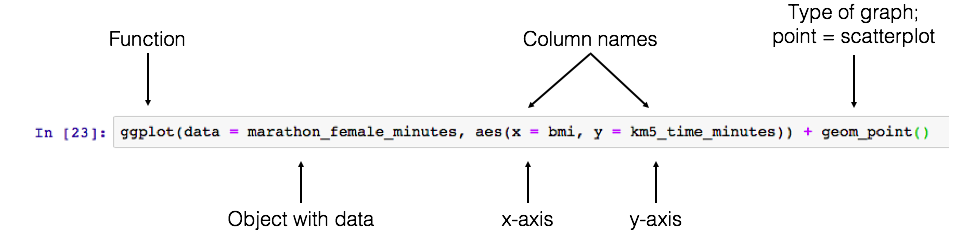
\includegraphics{images/ws1_ggplot_female.png}
\caption{ws1\_ggplot\_female.png}
\end{figure}

    \begin{Verbatim}[commandchars=\\\{\}]
{\color{incolor}In [{\color{incolor}55}]:} \PY{c+c1}{\PYZsh{} code to set\PYZhy{}up plot size}
         \PY{k+kn}{library}\PY{p}{(}repr\PY{p}{)}
         \PY{k+kp}{options}\PY{p}{(}repr.plot.width\PY{o}{=}\PY{l+m}{4}\PY{p}{,} repr.plot.height\PY{o}{=}\PY{l+m}{3}\PY{p}{)}
\end{Verbatim}


    \begin{Verbatim}[commandchars=\\\{\}]
{\color{incolor}In [{\color{incolor}56}]:} \PY{c+c1}{\PYZsh{} Run this cell to create a scatterplot of BMI against the time it took to run 5 kilometers. }
         ggplot\PY{p}{(}data \PY{o}{=} marathon\PYZus{}minutes\PY{p}{,} aes\PY{p}{(}x \PY{o}{=} bmi\PY{p}{,} y \PY{o}{=} km5\PYZus{}time\PYZus{}minutes\PY{p}{)}\PY{p}{)} \PY{o}{+} geom\PYZus{}point\PY{p}{(}\PY{p}{)}
\end{Verbatim}


    \begin{Verbatim}[commandchars=\\\{\}]
Warning message:
“Removed 160 rows containing missing values (geom\_point).”
    \end{Verbatim}

    
    
    \begin{center}
    \adjustimage{max size={0.9\linewidth}{0.9\paperheight}}{output_121_2.png}
    \end{center}
    { \hspace*{\fill} \\}
    
    \textbf{Question 7.13} Looking at the graph above, choose a statement
above that most reflects what we see?

A. There may be a postitive trend/relationship between 5 km run time and
body mass index; as the value for for body mass index increases, so does
the time it takes to run 5 km.

B. There may be a negative trend/relationship between 5 km run time and
body mass index; as the value for for body mass index increases, the
time it takes to run 5 km decreases.

C. There appears to be no trend/relationship between 5 km run time and
body mass index; as the value for for body mass index increases we see
neither an increase or decrease in the time it takes to run 5 km.

*Assign your answer to an object called \texttt{answer7.13}.

    \begin{Verbatim}[commandchars=\\\{\}]
{\color{incolor}In [{\color{incolor}57}]:} \PY{c+c1}{\PYZsh{} Assign your answer to an object called: answer7.13}
         \PY{c+c1}{\PYZsh{} Make sure the correct answer is an uppercase letter. }
         \PY{c+c1}{\PYZsh{} Surround your answer with quotation marks.}
         \PY{c+c1}{\PYZsh{} Replace the fail() with your answer. }
         
         \PY{c+c1}{\PYZsh{}\PYZsh{}\PYZsh{} BEGIN SOLUTION}
         answer7.13 \PY{o}{\PYZlt{}\PYZhy{}} \PY{l+s}{\PYZdq{}}\PY{l+s}{A\PYZdq{}}
         \PY{c+c1}{\PYZsh{}\PYZsh{}\PYZsh{} END SOLUTION}
\end{Verbatim}


    \begin{Verbatim}[commandchars=\\\{\}]
{\color{incolor}In [{\color{incolor}58}]:} test\PYZus{}that\PY{p}{(}\PY{l+s}{\PYZsq{}}\PY{l+s}{Solution is incorrect\PYZsq{}}\PY{p}{,} \PY{p}{\PYZob{}}
             expect\PYZus{}match\PY{p}{(}digest\PY{p}{(}answer7.13\PY{p}{)}\PY{p}{,} \PY{l+s}{\PYZsq{}}\PY{l+s}{75f1160e72554f4270c809f041c7a776\PYZsq{}}\PY{p}{)}
         \PY{p}{\PYZcb{}}\PY{p}{)}
         \PY{k+kp}{print}\PY{p}{(}\PY{l+s}{\PYZdq{}}\PY{l+s}{Success!\PYZdq{}}\PY{p}{)}
\end{Verbatim}


    \begin{Verbatim}[commandchars=\\\{\}]
[1] "Success!"

    \end{Verbatim}

    The code we listed above for graphics barely scratches the surface of
what ggplot, and R as a whole, are capable of. Not only are there far
more choices about the kinds of plots available, but there are many,
many options for customizing the look and feel of each graph. You can
choose the font, the font size, the colors, the style of the axes, etc.

Let's dig a little deeper into just a couple of options that you can add
to any of your graphs to make them look a little better. For example,
you can change the text of the x-axis label or the y-axis label by using
\texttt{xlab("")} or \texttt{ylab("")}. Let's do that for the
scatterplot to make the labels easier to read.

    \begin{Verbatim}[commandchars=\\\{\}]
{\color{incolor}In [{\color{incolor}59}]:} \PY{c+c1}{\PYZsh{} Run this cell. }
         \PY{c+c1}{\PYZsh{} You can replace the axes with whatever you wish to label. }
         \PY{c+c1}{\PYZsh{} After running the cell once, try changing the axes to something else. }
         
         ggplot\PY{p}{(}data \PY{o}{=} marathon\PYZus{}minutes\PY{p}{,} aes\PY{p}{(}x \PY{o}{=} bmi\PY{p}{,} y \PY{o}{=} km5\PYZus{}time\PYZus{}minutes\PY{p}{)}\PY{p}{)} \PY{o}{+} geom\PYZus{}point\PY{p}{(}\PY{p}{)} \PY{o}{+} 
         xlab\PY{p}{(}\PY{l+s}{\PYZdq{}}\PY{l+s}{Body Mass Index\PYZdq{}}\PY{p}{)} \PY{o}{+} ylab\PY{p}{(}\PY{l+s}{\PYZdq{}}\PY{l+s}{5km run time (minutes)\PYZdq{}}\PY{p}{)}
\end{Verbatim}


    \begin{Verbatim}[commandchars=\\\{\}]
Warning message:
“Removed 160 rows containing missing values (geom\_point).”
    \end{Verbatim}

    
    
    \begin{center}
    \adjustimage{max size={0.9\linewidth}{0.9\paperheight}}{output_126_2.png}
    \end{center}
    { \hspace*{\fill} \\}
    
    \subsection{Attributions}\label{attributions}

\begin{itemize}
\tightlist
\item
  UC Berkley \href{https://github.com/data-8/data8assets}{Data 8 Public
  Materials}
\end{itemize}


    % Add a bibliography block to the postdoc
    
    
    
    \end{document}
